\documentclass{report}

\usepackage[italian]{babel}
\usepackage[a4paper,top=2cm,bottom=2cm,left=3cm,right=3cm,marginparwidth=1.75cm]{geometry}

\usepackage{amsmath}
\usepackage{graphicx}
\usepackage[colorlinks=true, allcolors=blue]{hyperref}

\graphicspath{{./images/}}

\renewcommand{\baselinestretch}{1.3}

\title{Elaborato di Ingegneria del Software}
\author{Claudia Manfredi\\Mattia Pavlovic\\Elena Tonini}
\date{A.A. 2021/22}

\begin{document}
\maketitle
\tableofcontents

\chapter{Specifiche tecniche}
\section{Specifiche}

Si desidera realizzare, secondo un processo di sviluppo incrementale/iterativo, un sistema software di supporto al baratto di articoli (dotati di consistenza fisica) riconducibili a un insieme prefissato (non vuoto) di categorie. L’applicazione può essere adottata da varie organizzazioni, che sovrintendono al baratto di categorie diverse di articoli e/o operano su piazze diverse.

L’applicazione prevede due tipologie di utente, il \textit{configuratore} e il \textit{fruitore}.

Il primo è un esponente dell’organizzazione che, attraverso l’applicazione software, sovrintende agli scambi di beni senza uso di denaro; egli è deputato alla descrizione delle categorie di articoli scambiabili e può ottenere informazioni relative agli attuali baratti potenziali o a quelli già avvenuti.

Il secondo tipo di utente è una persona che si rivolge all’applicazione per prendere visione degli articoli pubblicati da altri (fruitori) come barattabili ed eventualmente effettuare degli scambi. Egli deve compilare dei campi atti a descrivere ciascun articolo che intende barattare.

Dopo avere descritto almeno un articolo, il fruitore può (ma non deve necessariamente) avanzare la proposta di barattare un suo articolo con quello di un altro fruitore così come rispondere alla proposta di baratto avanzata da un altro fruitore.

Si assume che le due parti coinvolte in un baratto si incontrino poi di persona al fine di scambiarsi i due articoli oggetto del baratto stesso.

Si noti che un fruitore può anche non descrivere mai alcun articolo, limitandosi a scorrere le descrizioni di articoli pubblicate dagli altri fruitori.


\section{Generalità}

L’applicazione è tesa a supportare il baratto di articoli (dotati di consistenza fisica) afferenti ad alcune categorie stabilite dal configuratore, a ciascuna delle quali corrisponde un insieme specifico di campi atti a descrivere ogni articolo (che si intende barattare) appartenente alla categoria stessa.

Ogni singola categoria è dotata di un \textit{nome} e di una \textit{descrizione}, entrambe stringhe in linguaggio naturale volte a esplicare il significato della categoria stessa.

Per esempio, il nome di una categoria può essere “Libro” e la sua descrizione “Opera cartacea stampata”.

Una categoria può articolarsi in due o più (sotto)categorie, a loro volta suddivisibili ricorsivamente, e così via, secondo una \textit{gerarchia} ad albero.

Ad esempio, la radice di una gerarchia può essere la categoria “Libro” ed essa può articolarsi nelle (sotto)categorie “Romanzo”, “Saggio”, “Opera a fumetti”, “Numero di un fumetto periodico” e “Testo scolastico”. A sua volta la categoria “Romanzo” può articolarsi nelle (sotto)categorie “Romanzo di letteratura italiana” e “Romanzo di letteratura straniera”, ecc.

Il nome di ciascuna categoria è unico all’interno della gerarchia di appartenenza.\newline

N.B. Non si deve erroneamente pensare che una gerarchia definisca ontologicamente un concetto (quello relativo alla radice), declinandolo in tutte le sfumature possibili. La gerarchia comprende invece solo le categorie che sono di interesse ai fini delle operazioni di baratto che l’organizzazione che si è dotata dell’applicazione intende sostenere.\newline

La medesima applicazione può considerare più gerarchie. Vige il vincolo di unicità del nome di ciascuna categoria radice entro la totalità delle categorie radice di tali gerarchie.

Gli articoli da scambiare devono appartenere solo alle categorie foglia delle gerarchie considerate.

A ciascuna categoria (a qualsiasi livello essa si collochi entro la gerarchia di appartenenza) compete inoltre un insieme (eventualmente vuoto) di \textit{campi nativi}, la compilazione di ciascuno dei quali da parte del fruitore è obbligatoria o facoltativa.

Di seguito, la compilazione di un campo che non è esplicitamente indicata come obbligatoria è da intendersi come facoltativa.

Ogni categoria radice è dotata almeno dei seguenti due campi nativi:
\begin{itemize}
  \item Stato di conservazione: a compilazione obbligatoria. Impone al fruitore di comunicare lo stato di conservazione e usura in cui si trova l’articolo proposto in baratto
  \item Descrizione libera: a compilazione facoltativa consente al fruitore di descrivere l’articolo proposto in baratto mediante un testo libero
\end{itemize}

Ciascuna categoria figlio eredita poi la totalità dei campi (nativi o ereditati) della categoria padre e i campi nativi devono avere un nome distinto da quello dei campi ereditati.\newline

Ad esempio, i campi nativi che competono alla categoria “Libro” (oltre ai due sopraindicati, comuni a tutte le categorie radice) potrebbero essere i seguenti:
\begin{itemize}
    \item Titolo a compilazione obbligatoria
    \item Autore/i a compilazione obbligatoria
    \item Casa editrice
    \item Anno di stampa
\end{itemize}

L’insieme dei campi nativi della categoria “Romanzo” potrebbe essere vuoto mentre quello della categoria “Romanzo di letteratura straniera” potrebbe essere dotato di un solo campo nativo:
\begin{itemize}
    \item Lingua di stampa a compilazione obbligatoria
\end{itemize}

Ogni articolo da barattare può essere descritto dal fruitore assegnando un valore a ciascuno dei campi (sia nativi sia derivati) che competono alla categoria foglia di appartenenza dello stesso.
Ogni valore è inserito dal fruitore sotto forma di una stringa di caratteri.\newline

Supponendo che un fruitore intenda proporre il baratto di un articolo appartenente alla categoria (foglia) “Romanzo di letteratura straniera”, egli potrebbe, ad esempio, compilare i campi come segue:
\begin{itemize}
    \item Stato di conservazione: nuovo
    \item Descrizione libera: volume a copertina flessibile mai sfogliato (doppione ricevuto in regalo)
    \item Titolo: A farewell to arms
    \item Autore/i: Ernest Hemingway
    \item Casa editrice: ''
    \item Anno di stampa: ''
    \item Lingua di stampa: Inglese
\end{itemize}


\section{Versioni}
Di seguito la presentazione delle versioni dell'applicazione, per ognuna delle quali vengono riportati i requisiti funzionali


\subsection{Versione 1}
La prima versione dell’applicazione consente l’accesso del solo configuratore.

Ogni configuratore effettua il primo accesso sfruttando credenziali predefinite (comunicate a ciascun nuovo configuratore che intende registrarsi), che lo qualificano come appartenente al gruppo (non vuoto, eventualmente individuale) dei configuratori dell’applicazione. 

Nell’ambito della sessione aperta al primo accesso egli dovrà immediatamente scegliere credenziali personali, da usare in tutti gli accessi successivi: solo a valle di tale scelta egli potrà operare sul back-end dell’applicazione. Lo username di ciascun configuratore lo individua univocamente.

La prima versione dell’applicazione consente al configuratore di: 
\begin{itemize}
    \item introdurre una nuova gerarchia di categorie
    \item dotare una nuova gerarchia di categorie di nome, descrizione e di tutti i suoi campi nativi, indicando l'eventuale obbligatorietà di ciascuno
    \item salvare in modo persistente tutte le informazioni di cui ai punti precedenti
    \item visualizzare ciascuna gerarchia presente e tutte le informazioni a corredo della stessa
\end{itemize}

\subsection{Versione 2}
La seconda versione dell’applicazione consente l’accesso anche al fruitore. 

Ogni fruitore deve scegliere al primo accesso le sue credenziali individuali, che gli consentiranno di operare sul front-end dell’applicazione. Lo username di ciascun fruitore individua univocamente il fruitore stesso (esso non deve coincidere con lo username di alcun altro fruitore né di alcun configuratore).

La seconda versione dell’applicazione dà la facoltà al configuratore di fissare il valore dei seguenti parametri:
\begin{itemize}
    \item Piazza: la città in cui avvengono gli scambi; per ipotesi, tale città è unica e, una volta stabilita, non può più cambiare;
    \item Luoghi: alcuni luoghi (al limite uno solo) in cui tali scambi sono effettuati;
    \item Giorni: il giorno o i giorni della settimana in cui gli scambi possono avere luogo;
    \item Intervalli orari: gli intervalli orari (almeno uno) entro cui effettuare gli scambi, dove i soli orari in corrispondenza dei quali si possono fissare appuntamenti finalizzati allo scambio di articoli fra le due parti coinvolte in un baratto sono quelli dello scoccare dell’ora e della mezz’ora;
    \item Scadenza: il numero massimo di giorni entro cui un fruitore può accettare una proposta di scambio avanzata da un altro fruitore.
\end{itemize}
Ad esempio, il configuratore può fissare i seguenti valori:
\begin{itemize}
    \item Piazza: Brescia
    \item Luoghi: Piazzale Kossuth, zona nord del parcheggio
    \item Giorni: giovedì, venerdì
    \item Intervalli orari: 17.00-19.30
\end{itemize}
Si noti che l’intervallo orario sopra esemplificato implica che gli appuntamenti possano essere fissati (solo) alle ore 17.00, 17.30, 18.00, 18.30, 19.00 e 19.30.\newline

Infine, la seconda versione dell’applicazione visualizza, a beneficio del fruitore, il nome e la descrizione delle categorie radice di tutte le gerarchie, nonché la piazza, i luoghi, i giorni e gli intervalli orari in cui sono possibili gli scambi.

\subsection{Versione 3}
La terza versione consente al fruitore di pubblicare le informazioni circa un articolo che egli intende barattare.

A tal fine il fruitore deve individuare (magari con l’aiuto dell’applicazione) la \textit{categoria foglia} di appartenenza e compilare i campi (nativi ed ereditati) relativi alla stessa. 

L’applicazione accetta la pubblicazione relativa a un articolo solo se sono stati compilati almeno i campi obbligatori di pertinenza. 

Le informazioni circa la categoria di appartenenza di tale articolo e il contenuto della pubblicazione accettata (valori dei campi), nonché il collegamento fra la stessa e lo username del fruitore autore di suddetta pubblicazione, vengono salvati in modo persistente. 

Una pubblicazione accettata rappresenta un’offerta di baratto che si trova nello stato di \textit{Offerta aperta}. Il fruitore autore di una \textit{Offerta aperta} non può modificare le informazioni fornite in merito all’articolo da barattare, egli può però ritirare tale offerta, trasformandone così lo stato in quello di \textit{Offerta ritirata}.

L’applicazione deve mantenere traccia dei passaggi di stato subiti da un’offerta, salvando le informazioni relative a tali passaggi in modo persistente. 

In ogni momento, il configuratore e così pure il fruitore può indicare una categoria (foglia) di una qualsiasi gerarchia e visualizzare tutte le attuali \textit{Offerte aperte} relative a tale categoria. Inoltre, il fruitore può visualizzare tutte le \textit{Offerte aperte} e le \textit{Offerte ritirate} di cui è autore, indipendentemente dalla categoria di appartenenza.

\subsection{Versione 4}
Questa versione consente a una coppia di fruitori di accordarsi per un baratto. 

Il fruitore autore di una \textit{Proposta aperta} (relativa a un articolo A) può infatti scegliere un’altra \textit{Proposta aperta} (relativa a un articolo B) – ma solo se di questa non è autore ed essa appartiene alla stessa categoria foglia. 
In tal modo il fruitore autore della prima proposta indica la sua disponibilità ad accettare B in cambio di A. In questo caso l’offerta relativa ad A passa nello stato di \textit{Offerta accoppiata}, lo stato dell’offerta relativa a B cambia in quello di \textit{Offerta selezionata} e viene creato un collegamento fra le due offerte.

Se il fruitore autore di una \textit{Offerta selezionata} non risponde alla proposta del fruitore autore della corrispondente \textit{Offerta accoppiata} entro il numero di giorni prestabilito (pari al valore del parametro di configurazione “Scadenza”), allo scadere di tale termine entrambe le offerte ritornano allo stato di \textit{Offerta aperta}. 

Il fruitore che invece risponde (necessariamente affermativamente) alla proposta del fruitore autore dell’\textit{Offerta accoppiata} corrispondente entro il numero di giorni prestabilito, nella risposta deve indicare gli estremi (luogo, data e ora) di un possibile appuntamento (in occasione del quale effettuare lo scambio dei due oggetti). 

Nel momento in cui tale risposta è inviata, entrambe le offerte coinvolte passano allo stato di \textit{Offerta in scambio}, mantenendo sempre traccia l’una dell’altra. 

Il fruitore autore della (ex) \textit{Offerta accoppiata} deve ora rispondere, entro il numero massimo di giorni (il solito valore del parametro di configurazione “Scadenza”), accettando tale appuntamento o scartandolo e proponendone uno alternativo (in altro luogo e/o data e/o ora, fra quelli consentiti), e così via. 

Lo scambio di proposte di appuntamenti prosegue fino a quando si verifica una di queste condizioni: 
\begin{itemize}
    \item una delle due parti accetta l’appuntamento proposto dall’altra,
    \item la parte che deve rispondere alla proposta di appuntamento non lo fa entro i termini stabiliti.
\end{itemize}
Se si verifica la prima condizione, l’una e l’altra \textit{Offerta in scambio} passano nello stato di \textit{Offerta chiusa}.\newline
Se invece si verifica la seconda condizione, l’una e l’altra \textit{Offerta in scambio} recidono il collegamento reciproco e passano nello stato di \textit{Offerta aperta}.\newline

Ciascun fruitore può visualizzare tutte le offerte di cui è autore, indipendentemente dallo stato e dalla categoria di appartenenza di ognuna.\newline
Inoltre, per ciascuna \textit{Offerta in scambio} di cui è autore, egli può visualizzare l’ultima risposta fornita dall’autore dell’offerta a essa collegata. \newline

Si noti che, al passaggio di un’offerta dallo stato di \textit{Offerta aperta} a quello di \textit{Offerta selezionata} (e, analogamente, al passaggio di un’offerta dallo stato di \textit{Offerta accoppiata} allo stato di \textit{Offerta in scambio}), l’autore della prima si rende conto del fatto che è invitato a rispondere al fruitore autore della seconda – e se ne rende conto proprio in virtù di tale passaggio (di cui può acquisire consapevolezza solo se accede all’applicazione e visualizza le offerte di sua pertinenza), non già perché gli viene inviato un messaggio (ad esempio, di posta elettronica). 

Parimenti, quando sopra si parla di “invio” di una risposta da parte di un fruitore, si intende che tale fruitore può “allegare” la risposta, cioè la proposta di un appuntamento, a un’\textit{Offerta selezionata} oppure a un’\textit{Offerta in scambio} di cui è autore e che suddetta risposta è visualizzabile dal fruitore autore dell’offerta collegata. 
Quest’ultimo, però, si rende conto di quale appuntamento è stato proposto solo se accede all’applicazione e richiede la visualizzazione della risposta “allegata” all’offerta collegata. 

Quindi, la comunicazione non avviene mai attraverso messaggi (ad esempio, di posta elettronica) inviati esplicitamente da un fruitore a un altro (i fruitori ignorano lo username degli altri fruitori e non hanno modo di contattarli direttamente). \newline

Il configuratore può indicare una categoria foglia di una gerarchia e visualizzare le attuali Offerte in scambio nonché le Offerte chiuse relative ad articoli di tale categoria. 

\subsection{Versione 5}
La quinta versione consente al configuratore di importare gli ingressi del back-end dell’applicazione, ovvero gerarchie delle categorie e valori dei parametri di configurazione, in modalità batch (cioè attraverso uno o più file di input) anziché in modalità interattiva.

\section{Requisiti non funzionali}
\begin{itemize}
    \item Il modello di processo da adottare è incrementale/iterativo.
    \item Il linguaggio di programmazione da utilizzare è Java.
    \item L’architettura esterna da realizzare per l’applicazione è stand alone.
    \item Requisito non prescrittivo ma importante in sede di valutazione è l’impiego di precondizioni, postcondizioni e invarianti di classe entro il codice Java.
    \item Non è richiesta la creazione di una interfaccia utente grafica (tuttavia è bene che l’architettura interna sia progettata in modo da ridurre gli effetti collaterali e lo sforzo connesso al cambiamento se in futuro il sistema di interazione testuale fosse sostituito da una GUI).
    \item Non è richiesto l’impiego di alcun DBMS (Data Base Management System).
\end{itemize}

\section{Nota}
Ogni versione da produrre estende le funzionalità della precedente, senza modificarle.\newline

Nei requisiti sopra enunciati si sono ignorati i possibili aspetti legali connessi alla gestione di un’applicazione volta a supportare il baratto di articoli, all’uso della stessa e al baratto vero e proprio. 

È evidente che ogni applicazione che operi nel mondo reale deve rispettare la legislazione del Paese in cui viene utilizzata. Tale legislazione potrebbe imporre, per esempio, che ciascun fruitore fornisca le sue generalità oppure che dichiari di essere maggiorenne, che autocertifichi che gli articoli proposti in baratto rientrano nella sua personale disponibilità e non sono frutto di attività illecite, ecc. 
Inoltre, le Offerte aperte dovrebbero essere pubblicate solo se non contengono (ad esempio, entro la descrizione dell’articolo mediante un testo libero) messaggi inaccettabili (perché offensivi o altro). 

Queste considerazioni mettono in luce l’opportunità di un ulteriore tipo di utente, il moderatore, che dovrebbe effettuare controlli di questo genere (così come quelli volti a evitare truffe). 

La ragione per cui questa ulteriore figura di utente e tali controlli – essenziali in una applicazione professionale – sono stati ignorati è che l’applicazione che sarà realizzata è da intendere come il frutto di un esercizio, necessariamente di dimensioni limitate, e non è destinata a essere effettivamente installata e usata nella realtà quotidiana, come sottolineato dal requisito di adottare un’architettura esterna stand alone (mentre una applicazione che supporta il baratto nel mondo reale dovrebbe operare in rete). \newline

Per la stessa ragione non si è mai parlato del ritorno atteso da parte dell’organizzazione che, attraverso l’applicazione, sovrintende alle operazioni di baratto. Tale ritorno esula completamente dagli scopi didattici del progetto.\newline

Nelle pagine precedenti si è assunto che i valori dei campi atti a descrivere un articolo che un fruitore desidera scambiare siano solo stringhe di caratteri. 
Nel caso più generale, alcuni valori potrebbero essere di tipo diverso, talvolta anche enumerativo (con richiesta al fruitore di fornire risposte chiuse). Inoltre, potrebbe essere contemplato che il fruitore carichi opzionalmente dei file (ad esempio, una fotografia dell’articolo che intende scambiare). 

Quest’ultimo è uno scenario complesso, in cui il requisito di sicurezza gioca un ruolo di rilievo. Tale requisito, sempre più importante in un lavoro professionale, non è stato considerato nei limiti dell’esercizio proposto né il gruppo di lavoro deve tenerne conto. 

L’enfasi del progetto non è infatti sulla sicurezza, pertanto anche l’attribuzione di credenziali a configuratore e fruitore non è ritenuta un’operazione critica. \newline

L’interpretazione relativa alle “credenziali predefinite” comunicate a ciascun nuovo configuratore che intende registrarsi, di cui ai requisiti funzionali della prima versione, non è univoca. 
Secondo l’interpretazione più semplice – e meno sicura – tali credenziali sono uniche e immutabili, stabilite al momento dell’installazione dell’applicazione. 
Un’interpretazione più complessa è quella secondo cui le credenziali predefinite sono diverse per ciascun configuratore che intende registrarsi. 
In questo caso, al primo configuratore che intende registrarsi vengono comunicate credenziali predefinite stabilite al momento dell’installazione dell’applicazione mentre a ciascuno di quelli successivi vengono comunicate nuove credenziali, fissate di volte in volta da un configuratore già registrato. Questa soluzione è più sicura ma non ne è richiesta la realizzazione.\newline

Secondo la trattazione precedente, il baratto è consentito solo fra articoli afferenti alla medesima categoria (foglia). 
In futuro si potrebbe consentire il baratto anche fra articoli di categorie compatibili, dove la compatibilità è stabilita a priori dal configuratore e salvata permanentemente.\newline

Tutte le versioni dell’applicazione attualmente previste assumono che ciascuna gerarchia di categorie, una volta introdotta dall’utente, sia immutabile (e pertanto è molto importante che tale gerarchia sia stata congegnata con attenzione). 
In futuro si potrebbe permettere l’estensione di una gerarchia attraverso l’aggiunta di sottoalberi. 
Se il padre della radice del sottoalbero da aggiungere è una categoria foglia, l’intervento sulla gerarchia comporta effetti collaterali sulle offerte non ancora chiuse né ritirate che cadono in tale categoria. \newline

I requisiti non funzionali non impongono alcuna tecnologia da utilizzare per la memorizzazione persistente dei dati (categorie, valori di configurazione, offerte e relativi passaggi di stato) né per l’importazione (non interattiva) degli input del back-end. 
Per quanto riguarda la prima, la scelta dei progettisti potrebbe cadere banalmente sulla serializzazione di oggetti. 
Per quanto riguarda la seconda, esistono più soluzioni, fra cui l’impiego di file di testo aventi una sintassi definita appositamente dai progettisti stessi (ad esempio, file in formato CSV o JSON o XML ...). Si noti che tali file potrebbero essere adottati anche per il salvataggio.\newline

I requisiti (funzionali e non) delle cinque versioni dell’applicazione da realizzare sono deliberatamente espressi a un alto livello di astrazione (ad esempio, non si è parlato esplicitamente di possibili conseguenze – che comunque non è necessario siano gestite – della modifica dei valori dei parametri di configurazione, né si è fissato – e non è indispensabile farlo – un numero massimo di tentativi entro cui le due parti di un baratto devono convergere nello stabilire luogo, data e ora dell’incontro in cui avviene lo scambio effettivo degli articoli; inoltre, non si è stabilita la lunghezza massima, in termini di numero di caratteri, delle stringhe attraverso cui il fruitore esprime il valore dei campi atti a descrivere un articolo) al fine di consentire agli ingegneri del software di fornire un’interpretazione personale, che comporta sempre l’aggiunta di ulteriori requisiti. \newline

Tali aggiunte devono essere chiaramente documentate.

\section{Richieste}
Agli studenti è richiesto di realizzare evolutivamente cinque versioni software che soddisfino i requisiti sopra esposti. Ogni gruppo (costituito al più da tre persone), dovrà: 
\begin{enumerate}
    \item per ogni versione, produrre la documentazione di progetto, contenente:
    \begin{itemize}
        \item casi d’uso (comprensivi dell’espressione di eventuali requisiti aggiuntivi), sia in forma testuale, sia in forma di diagramma UML; si invita a rendere evidenti a colpo l’occhio le integrazioni/modifiche apportate ai casi d’uso (testuali e grafici) della versione precedente per ottenere quelli della versione corrente;
        \item diagramma UML delle classi;
        \item diagrammi UML comportamentali (opzionali), e qualsiasi altra specifica ritenuta opportuna;
        \item la documentazione relativa alle cinque versioni deve essere raccolta in un unico file;
    \end{itemize}
    \item per l’ultima versione, redigere un unico manuale di installazione e uso (il cui contenuto potrebbe eventualmente divenire parte dell’help in linea dell’applicazione); si sottolinea la necessità di documentare accuratamente il da farsi al fine di importare nell’applicazione le gerarchie di categorie e i dati di configurazione;
    \item consegnare in formato elettronico quanto richiesto ai punti precedenti;
    \item per ogni versione, consegnare codice sorgente + codice interpretabile + (preferibilmente) codice eseguibile.
\end{enumerate}

\chapter{Documentazione}

\section{Versione 1}
\subsection{Casi d'uso}
In questa sezione sono riportati i casi d'uso relativi alla prima versione dell'applicazione, sia in forma testuale che come diagramma UML.\bigskip 

Nella descrizione testuale di tutti i casi d'uso eccetto "Creazione configuratore" e "Accesso configuratore" è lasciato sottinteso il fatto che l'utente debba aver effettuato l'accesso al proprio profilo prima di poter proseguire con l'interazione descritta dal caso d'uso considerato: la scelta relativa all'azione da effettuare e di conseguenza del caso d'uso a cui far riferimento avviene infatti tramite un menù presentato all'utente solo dopo aver effettuato l'accesso, pertanto non sarebbe possibile richiedere di effettuare alcuna operazione che non sia la creazione di un nuovo profilo Configuratore o l'accesso a un profilo già esistente prima che venga presentato il suddetto menù.\bigskip

Nella Tabella \ref{tab:Use Case 1.1} è riportato il caso d'uso testuale relativo all'accesso dell'utente configuratore al proprio profilo: l'utente interagisce con l'applicazione inserendo il proprio username e password; in questo caso d'uso, pertanto, è incluso il caso d'uso ``Creazione configuratore" che viene invocato nella situazione in cui non esista ancora alcun utente registrato.\bigskip

Nella Tabella \ref{tab:Use Case 1.2} è riportato il caso d'uso testuale relativo alla creazione di un nuovo profilo configuratore: l'utente riceve la comunicazione delle proprie credenziali temporanee, accede al proprio profilo e modifica le proprie credenziali a piacere (rispettando il vincolo relativo all'univocità dello username).\bigskip

Nella Tabella \ref{tab:Use Case 1.3} è riportato il caso d'uso testuale relativo alla creazione di una nuova gerarchia da parte dell'utente configuratore: l'utente, dopo aver effettuato l'accesso, interagisce con l'applicazione chiedendo di aggiungere nuove categorie oppure salvare la configurazione esistente; in questo caso d'uso, pertanto, sono inclusi i casi d'uso ``Aggiunta categoria" e ``Salvataggio dati", a cui si demandano i compiti relativi.\bigskip

Nella Tabella \ref{tab:Use Case 1.4} è riportato il caso d'uso testuale relativo alla Visualizzazione di tutte le gerarchie presenti all'interno dell'applicazione da parte dell'utente configuratore.\bigskip

Nella Tabella \ref{tab:Use Case 1.5} è riportato il caso d'uso testuale relativo all'aggiunta di una categoria a una gerarchia; si tratta di un caso d'uso incluso in quello relativo alla creazione di una gerarchia.\bigskip

Nella Tabella \ref{tab:Use Case 1.6} è riportato il caso d'uso testuale relativo al salvataggio dei dati introdotti nell'applicazione dall'utente configuratore.\bigskip

In Figura \ref{fig:Use Case 1} è riportato il diagramma UML dei casi d'uso relativo alla prima versione dell'applicazione. Dall'immagine possiamo ricavare facilmente che i casi d'uso \textit{sea-level}, ossia quelli corrispondenti agli obiettivi per cui l'utente interagisce con l'applicazione, sono:
\begin{itemize}
    \item Creazione di un nuovo profilo configuratore 
    \item Accesso a un profilo configuratore già esistente
    \item Creazione di una gerarchia di categorie
    \item Visualizzazione di tutte le gerarchie di categorie presenti nell'applicazione
    \item Salvataggio dei dati dell'applicazione
\end{itemize}
Alcuni di questi casi d'uso \textit{sea-level} sono interpretabili come casi d'uso \textit{fish-level} laddove vengano inclusi da un altro caso d'uso al fine del raggiungimento dell'obiettivo per cui l'utente interagisce con l'applicazione.

L'unico caso d'uso che ha natura esclusivamente \textit{fish-level} è quello relativo all'aggiunta di una nuova categoria a una gerarchia, in quanto esso è incluso nel caso d'uso "Creazione gerarchia". Inoltre, i casi d'uso "Creazione configuratore" e "Salvataggio dati" sono inclusi in altri casi d'uso \textit{sea-level}, pertanto possono essere visti anche come casi d'uso \textit{fish-level} oltre che \textit{sea-level}.

\begin{figure}[hb]
\centering
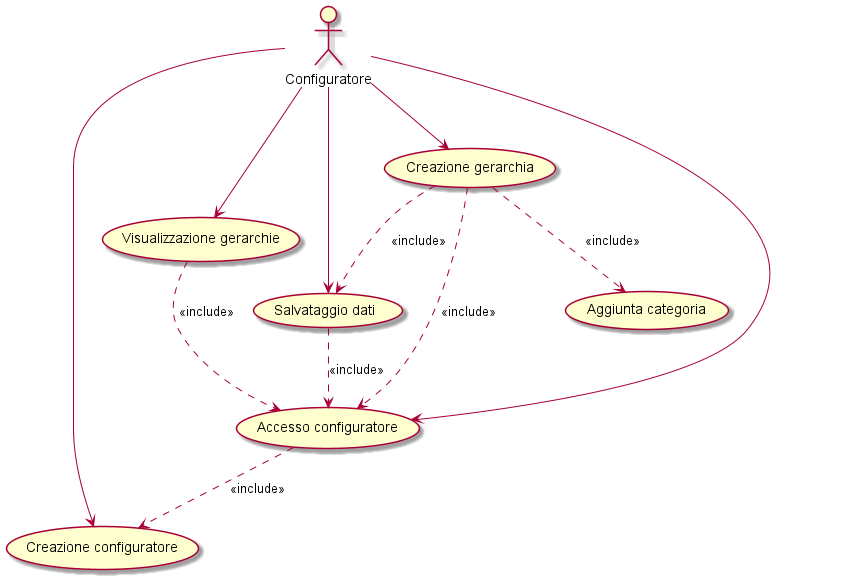
\includegraphics[width=0.9\textwidth]{imagesV1/Use case diagram-Version 1.0.png}
\caption{\label{fig:Use Case 1}Diagramma UML dei casi d'uso - Versione 1}
\end{figure}\bigskip
\newpage
\subsection{Diagramma UML delle classi}
In questa sezione sono stati riportati tre diagrammi delle classi: il primo, in Figura \ref{fig:Initial Class diagram}, rappresenta il diagramma delle classi realizzato come prototipo per la progettazione dell'applicazione, il secondo, in Figura \ref{fig:Class diagram}, rappresenta il diagramma delle classi effettivamente ottenuto a seguito della stesura del codice dell'applicazione, mentre il terzo, in Figura \ref{fig:Simplified Class Diagram} rappresenta una versione semplificata del diagramma delle classi. In quest'ultima versione, in particolare, sono state rimosse alcune dipendenze in modo tale da rendere la comprensione di alcune relazioni tra classi visivamente più agevole.

Si tenga inoltre conto del fatto che le classi:
\begin{itemize}
    \item CampoNativo
    \item Categoria
    \item Configuratore
    \item Gerarchia
    \item User
    \item UserDataStore
\end{itemize}
implementano l'interfaccia \texttt{Serializable}, nonostante tale relazione non sia esplicitamente riportata nei diagrammi delle classi al fine di semplificare il layout dei diagrammi stessi.

\begin{figure}[hb]
    \centering
    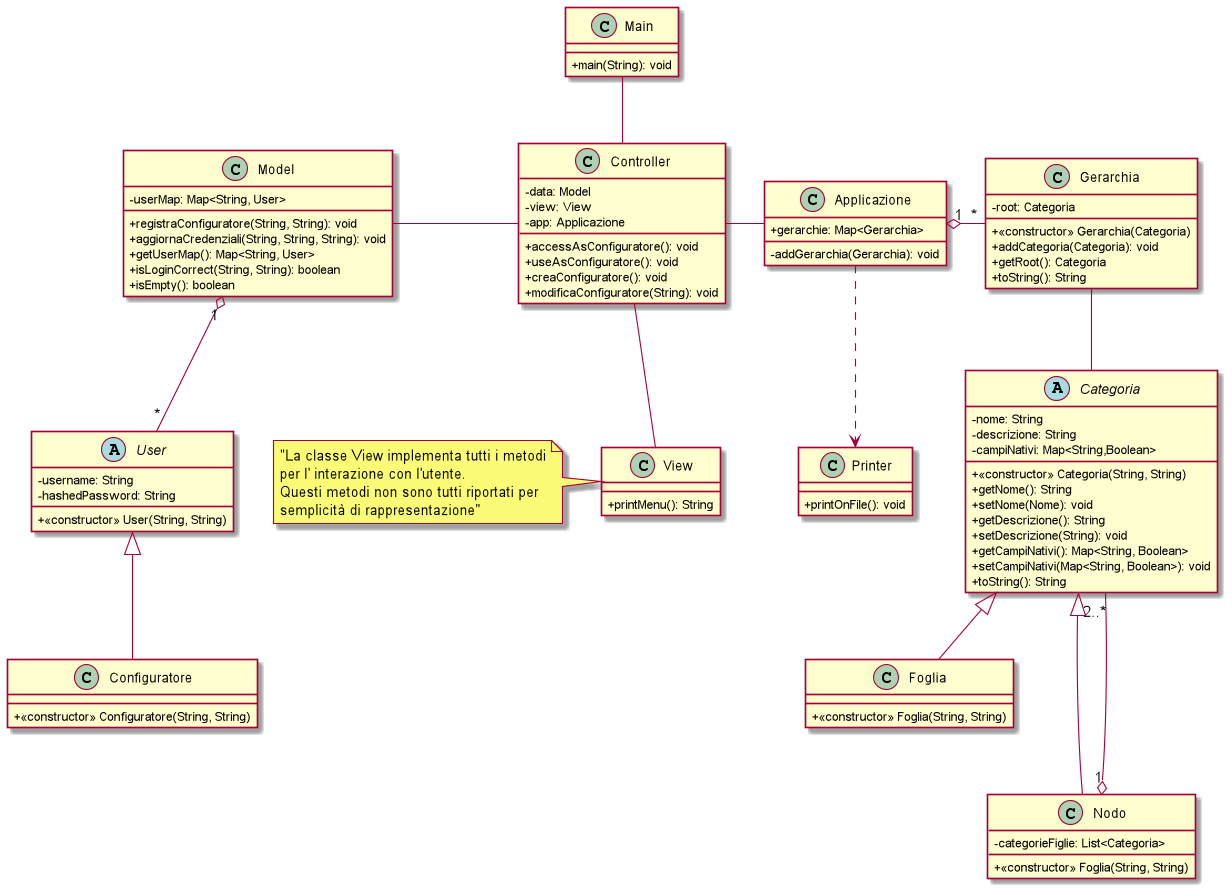
\includegraphics[width=\textwidth]{imagesV1/Initial class diagram - Version 1.0.png}
    \caption{\label{fig:Initial Class diagram}Prototipo di diagramma UML delle classi - Versione 1}
\end{figure}

\begin{figure}[h!]
    \centering
    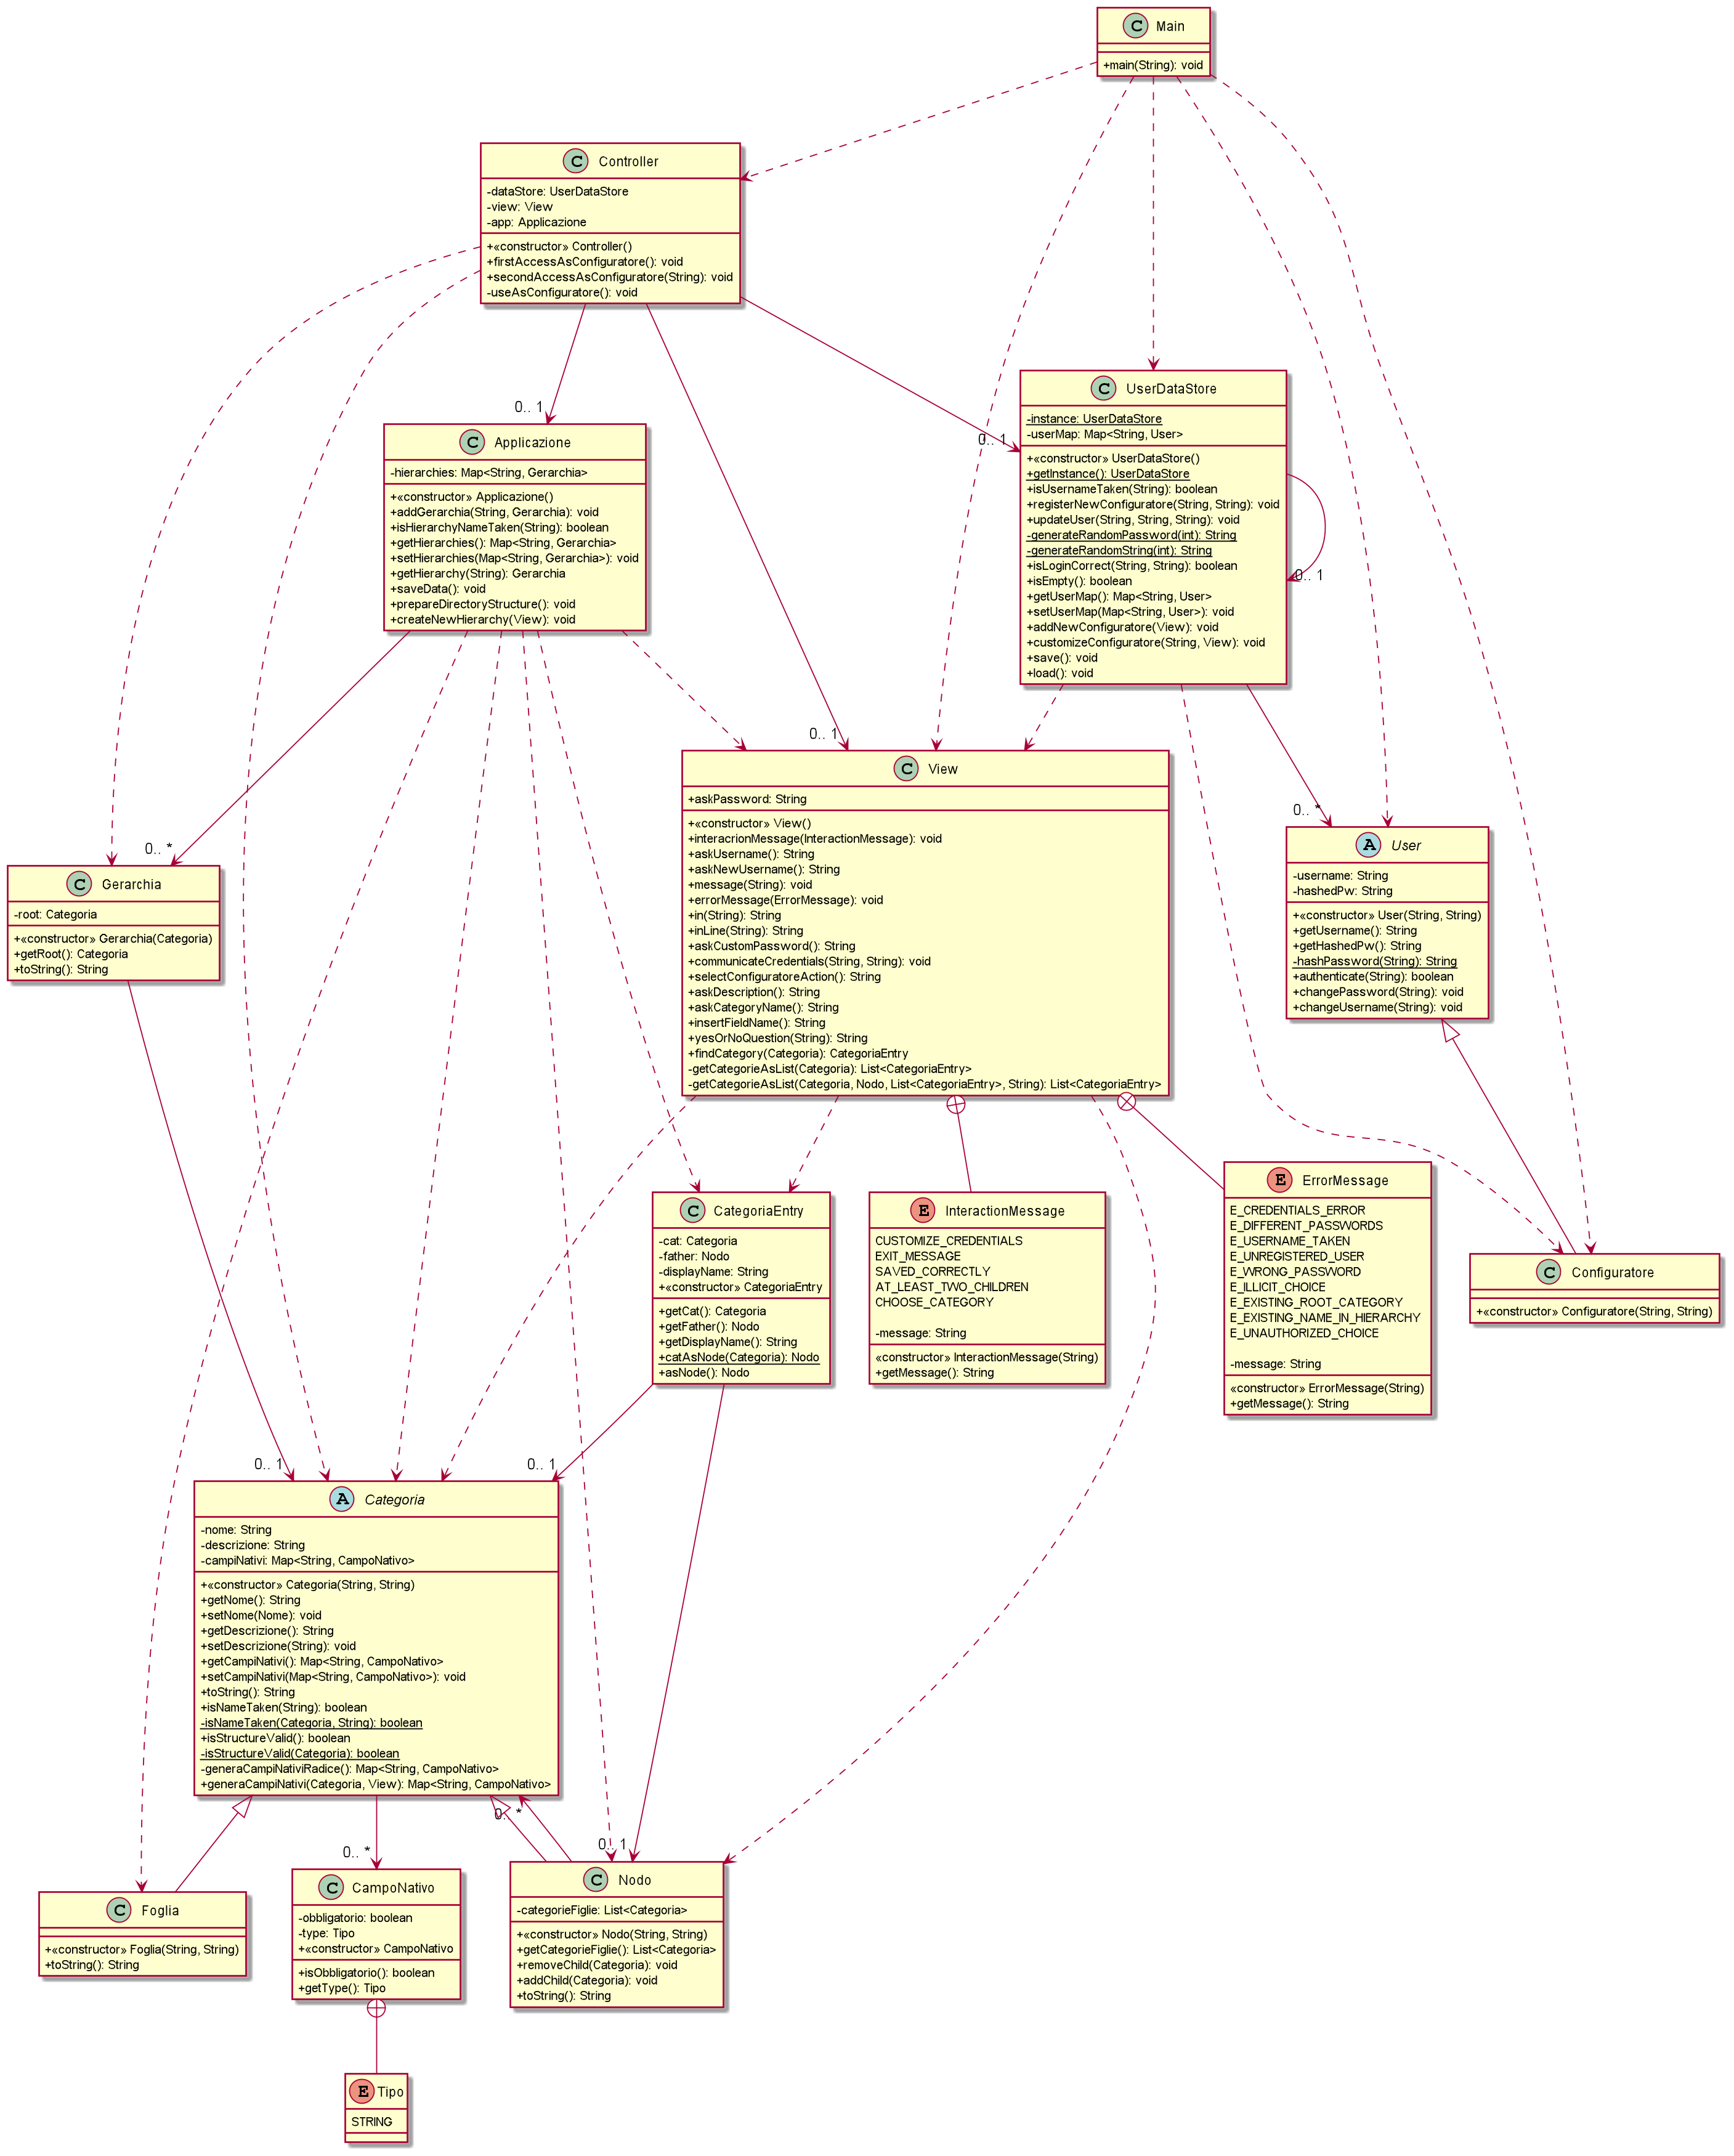
\includegraphics[width=\textwidth]{imagesV1/Class diagram-Version1.0.png}
    \caption{\label{fig:Class diagram}Diagramma UML delle classi - Versione 1}
\end{figure}    

La classe \texttt{View} contiene tutti i metodi (non indicati per esteso nel diagramma delle classi realizzato prima dell'effettiva stesura del codice) necessari per interagire e comunicare con l'utente, ricevendo i dati da lui inseriti oppure comunicando messaggi da parte del sistema.

La classe \texttt{Model}, presente con questo nome nell'UML iniziale ma rinominata \texttt{UserDataStore} nel codice finale, contiene i metodi necessari per la gestione dei dati relativi agli utenti che dovranno poi essere salvati in modo persistente. La classe ha il compito di gestire la registrazione di un nuovo utente Configuratore, l'aggiornamento delle credenziali e la verifica della correttezza delle informazioni introdotte in fase di login, oltre al salvataggio e al caricamento dei dati. 

La classe \texttt{User} è una classe astratta estesa dalla classe \texttt{Configuratore}: ogni Configuratore sarà dotato di username e password. La password, in particolare, viene salvata direttamente dopo aver effettuato l'hashing, in modo da garantire un livello di sicurezza basilare relativamente alle informazioni private degli utenti. La classe \texttt{User} è dotata di metodi per l'autenticazione dell'utente e per la modifica delle credenziali.

La classe \texttt{Applicazione} permette di tenere traccia delle gerarchie contenute nell'applicazione. 
Essa contiene infatti un metodo che verifica se il nome di una categoria radice di una gerarchia è già utilizzato dalla categoria radice di un'altra gerarchia, uno che permette di aggiungere una nuova gerarchia, metodi che permettono di ottenere le gerarchie presenti nell'applicazione o di assegnare loro i valori desiderati, metodi che permettono di salvare i dati contenuti nelle gerarchie e di caricare i dati salvati durante gli utilizzi precedenti dell'applicazione.

La classe \texttt{Gerarchia} permette di tenere traccia del contenuto di ogni gerarchia: ogni gerarchia è caratterizzata da una categoria radice che, a seconda che sia istanza della classe \texttt{Foglia} o \texttt{Nodo}, può avere o meno delle sottocategorie (a loro volta istanze della classe \texttt{Foglia} o \texttt{Nodo}). 

La classe \texttt{Categoria} è una classe astratta che è estesa dalla classe \texttt{Foglia} e dalla classe \texttt{Nodo}. Ogni categoria è dotata di nome obbligatorio, descrizione facoltativa e un insieme di campi nativi (due dei quali presenti di default per la categoria radice di una gerarchia) ereditati poi da ogni categoria figlia di un nodo.
La classe \texttt{Nodo}, in particolare, è dotata di una lista di categorie figlie che possono a loro volta essere foglie o nodi. Per questo motivo la classe \texttt{Nodo} è dotata di metodi che permettono di aggiungere o rimuovere una categoria figlia e di un metodo che permette di ottenere tutte le categorie figlie.

La classe \texttt{CampoNativo} tiene traccia dell'obbligatorietà della compilazione di un campo nativo o ereditato relativo a una categoria e del tipo del campo (di default si tratta di stringhe). 

La classe \texttt{CategoriaEntry} tiene traccia dell'associazione tra una categoria e la sua categoria padre; essa contiene pertanto i metodi necessari a recuperare le informazioni relative a tale relazione (percorso dalla categoria radice alla categoria corrente, categoria padre e categoria corrente) e dei metodi per trasformare una categoria da Foglia a Nodo e associarla alla propria categoria padre.

La classe \texttt{Controller} contiene metodi per consentire l'accesso a un profilo Configuratore, differenziando tra il caso di registrazione e quello di accesso standard. Ognuno di questi metodi richiama poi uno o più ulteriori metodi che permettono l'utilizzo delle funzionalità a cui l'utente è autorizzato ad accedere.

La classe \texttt{Main} contiene il solo metodo main che permette di interagire con l'applicazione selezionando l'azione da compiere tra accesso, registrazione o uscita dall'applicazione.

\begin{figure}[!]
    \centering
    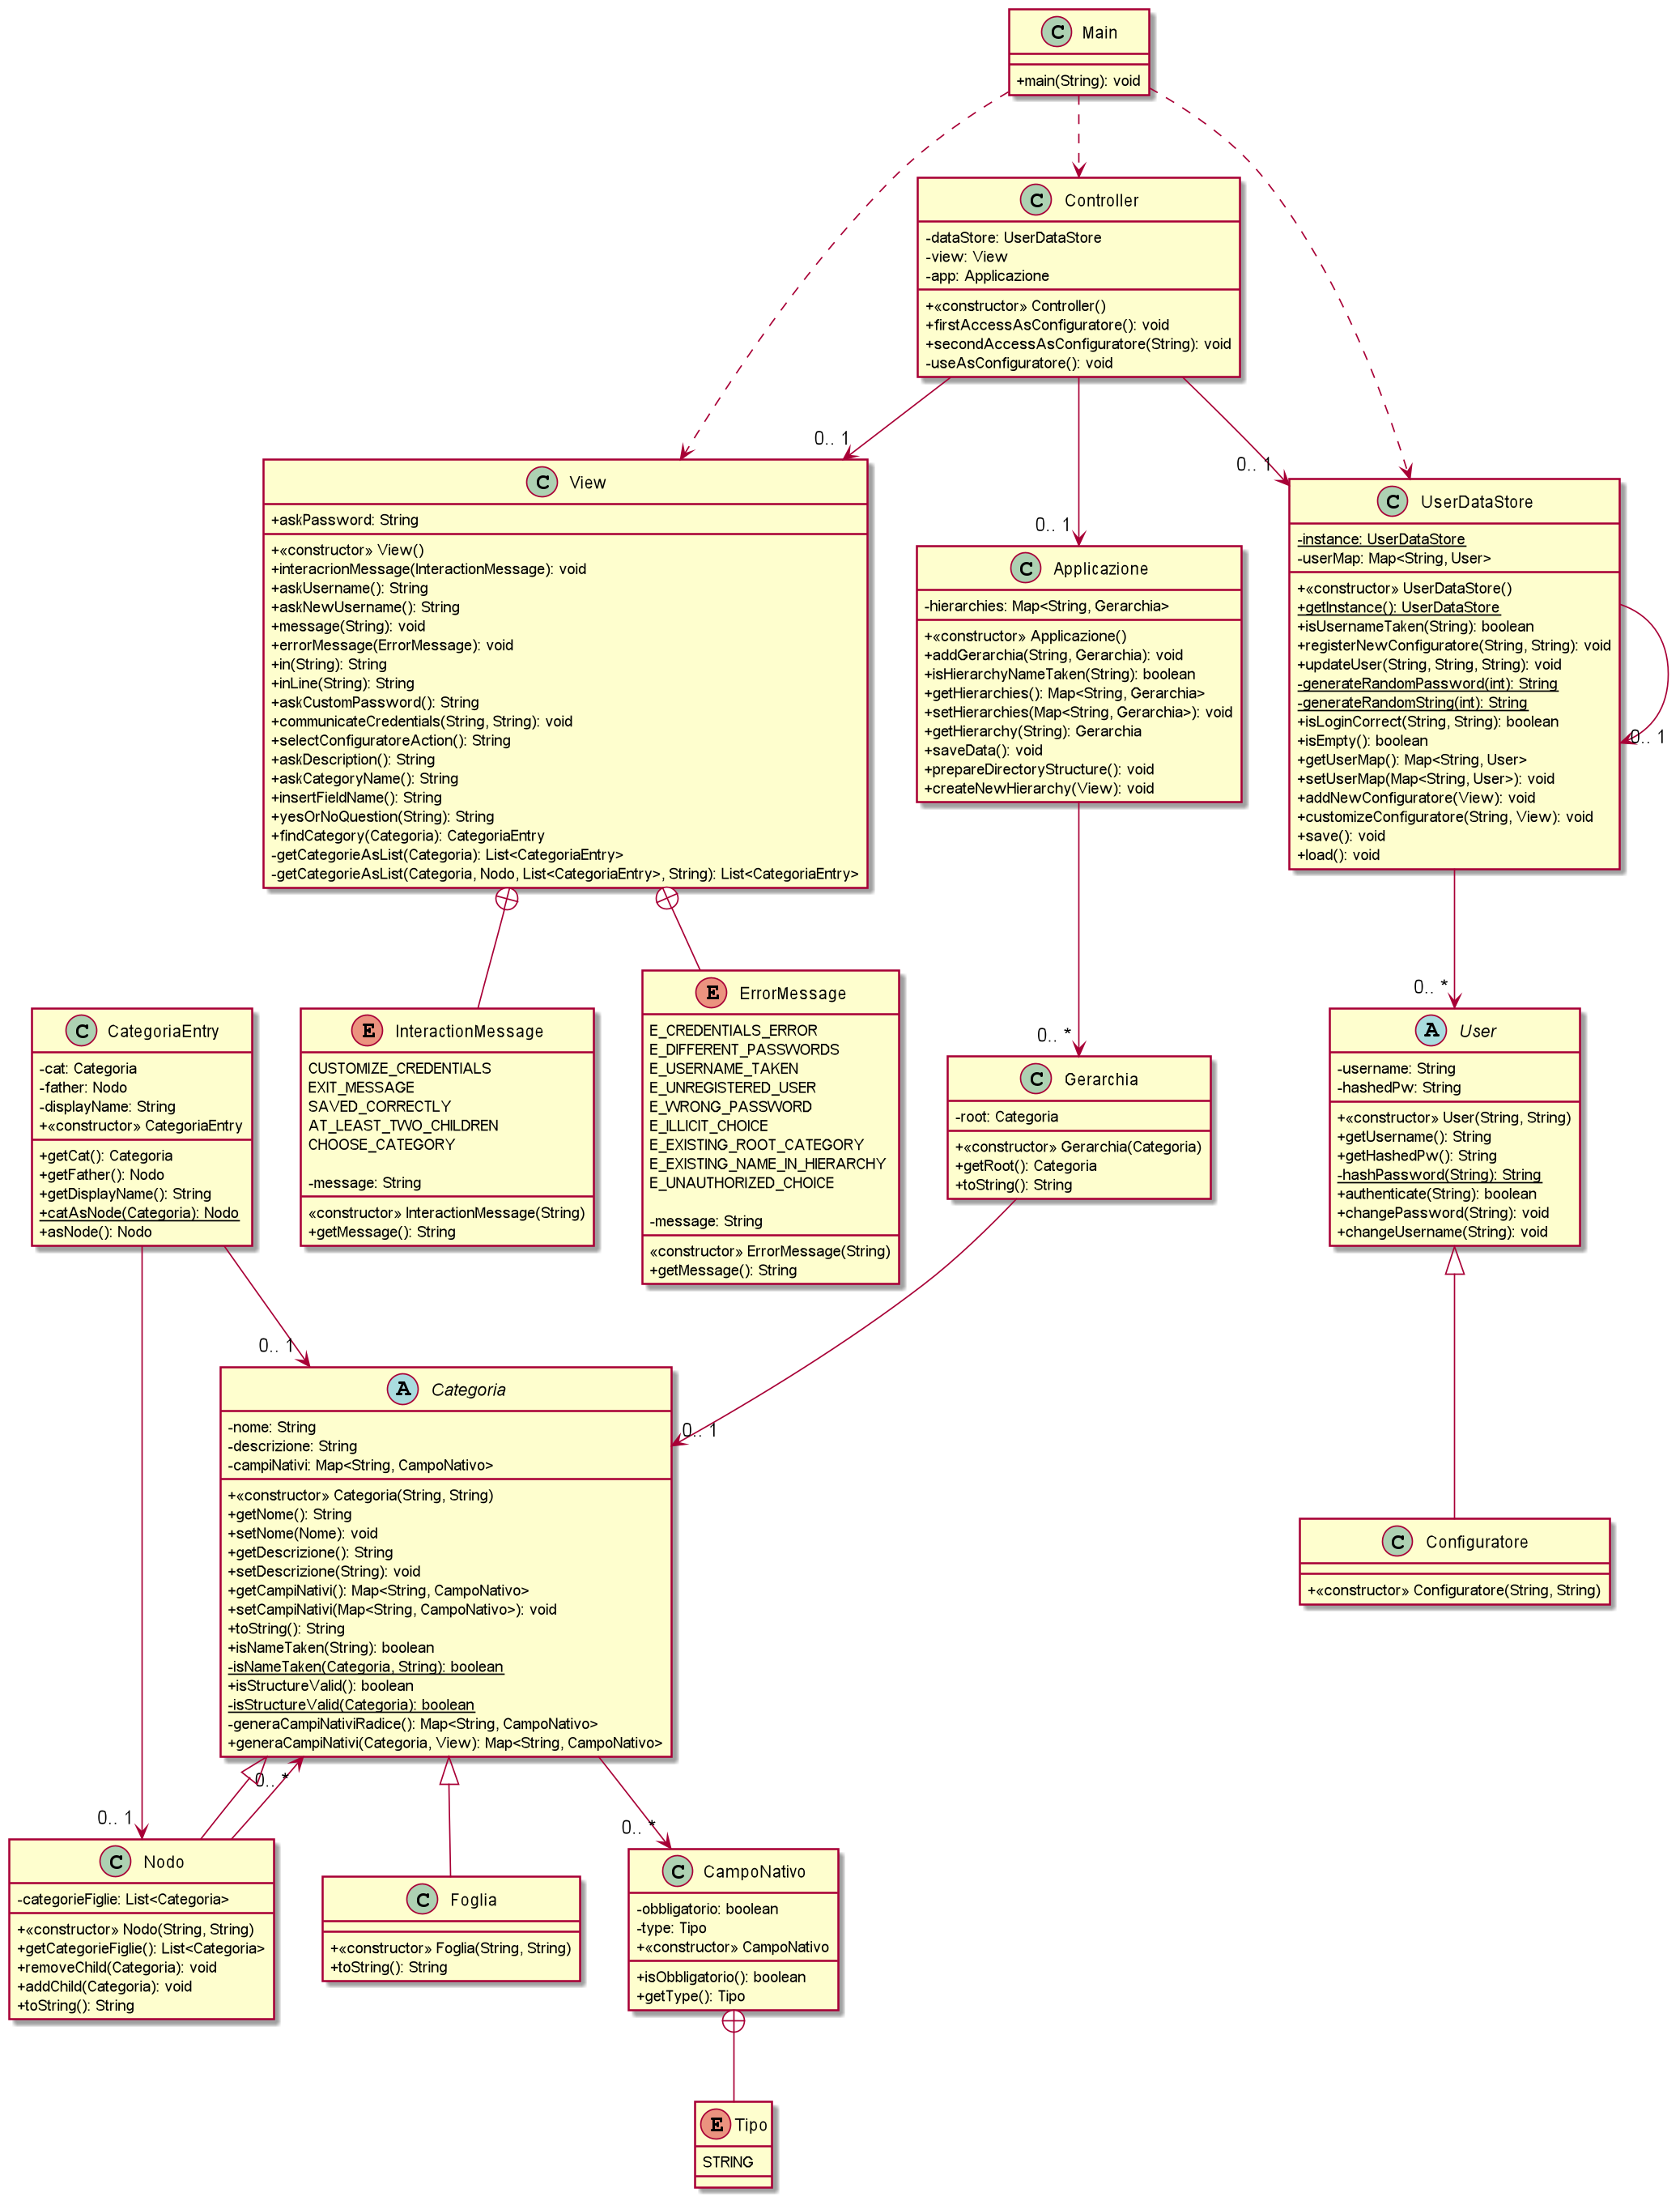
\includegraphics[width=\textwidth]{imagesV1/Class diagram simplified-Version1.0.png}
    \caption{\label{fig:Simplified Class Diagram}Diagramma UML delle classi semplificato - Versione 1}
\end{figure}
\newpage
\subsection{Diagrammi UML comportamentali}
In questa sezione sono riportati alcuni diagrammi comportamentali a corredo dei diagrammi dei casi d'uso e UML delle classi che illustrano il funzionamento della prima versione dell'applicazione.

I diagrammi UML riportati di seguito sono altamente descrittivi, in modo da essere utilizzabili per mostrare all'utente in maniera intuitiva il funzionamento dell'applicazione, pur rispettando le direttive UML.\bigskip

\textbf{Diagramma di sequenza: Accesso Configuratore}\newline
In Figura \ref{fig:Sequence diagram 1.1} è riportato il diagramma di sequenza che rappresenta gli step che caratterizzano l'interazione dell'utente con l'applicazione per consentire all'utente Configuratore di accedere all'applicazione.\newline Si presenta di seguito la descrizione ad alto livello delle azioni che si verificano in corrispondenza di ogni numero riportato sulle frecce:

\begin{enumerate}
    \item L'utente richiede di accedere al proprio profilo
    \item L'applicazione richiede all'utente di inserire il proprio username nell'interfaccia presentatagli
    \item L'utente inserisce il proprio username
    \item L'interfaccia comunica al Controller dell'applicazione lo username inserito dall'utente
    \item Il Controller verifica l'esistenza dello username all'interno dell'elenco degli utenti
    \item Se lo username esiste all'interno dell'elenco degli utenti il Controller manda un messaggio di conferma della correttezza dei dati inseriti all'interfaccia
    \item L'interfaccia dell'applicazione richiede all'utente la password
    \item L'utente inserisce la propria password
    \item L'interfaccia comunica al Controller dell'applicazione la password inserita dall'utente
    \item Il Controller verifica la correttezza della password
    \item Se la password è corretta il Controller comunica all'interfaccia che il login è stato effettuato correttamente
    \item L'interfaccia comunica all'utente che il login è stato effettuato correttamente
    \item Se la password è errata il Controller comunica all'interfaccia che il login è fallito
    \item L'interfaccia comunica all'utente che il login è fallito
    \item Se lo username è inesistente il Controller comunica all'interfaccia che il login è fallito
    \item L'interfaccia comunica all'utente che il login è fallito
\end{enumerate}

\begin{figure}[!]
\centering
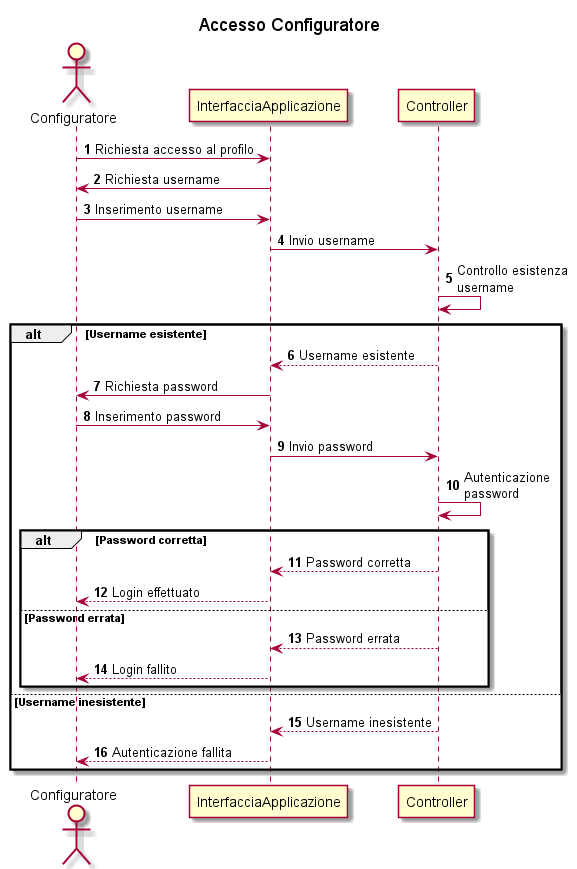
\includegraphics[width=0.6\textwidth]{imagesV1/Sequence diagram-Accesso configuratore-Accesso_Configuratore.png}
\caption{\label{fig:Sequence diagram 1.1}Diagramma di sequenza: Accesso configuratore - Versione 1}
\end{figure}\bigskip

\newpage
\textbf{Diagramma degli Stati: Ciclo di vita dell'utente Configuratore}\newline
In Figura \ref{fig:State diagram 1.1} è rappresentato il ciclo di vita dell'utente Configuratore: a seconda dell'azione che esso intraprende nei confronti dell'applicazione il Configuratore si trova in un determinato stato.\newline L'accesso all'applicazione può avvenire o in qualità di primo accesso oppure come accesso ordinario: nel caso si tratti di un primo accesso il configuratore si riconduce allo stato "CreazioneProfilo" in cui avviene la creazione di un nuovo profilo Configuratore a cui segue un necessario cambio delle credenziali, mentre nel caso si tratti di un login ordinario l'utente accede direttamente al menù principale. \newline 
In tutti i passaggi di stato si considera la situazione ideale in cui non vi siano errori nell'esecuzione delle operazioni. Nel caso in cui si verifichino errori di esecuzione allora è lasciato sottinteso il passaggio attraverso uno stato di Errore prima di tornare al menù principale.

\begin{figure}[b!]
\centering
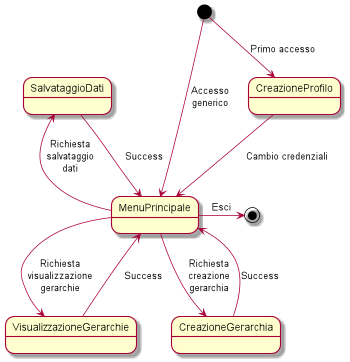
\includegraphics[width=0.7\textwidth]{imagesV1/State diagram - Version 1.0.png}
\caption{\label{fig:State diagram 1.1}Ciclo di vita del Configuratore - Versione 1}
\end{figure}\bigskip

\cleardoublepage
\section{Versione 2}
\subsection{Casi d'uso}
In questa sezione sono riportati i casi d'uso relativi alla seconda versione dell'applicazione, sia in forma testuale che come diagramma UML.\bigskip 

In questa sezione sono riportati anche i casi d'uso che non sono soggetti a modifiche nella transizione dalla prima alla seconda versione dell'applicazione, al fine di presentarne una descrizione completa della struttura e del funzionamento.\bigskip

I casi d'uso specifici della seconda versione e non presenti nella prima sono:
\begin{itemize}
    \item Creazione fruitore
    \item Accesso fruitore
    \item Visualizzazione Informazioni app
    \item Configurazione parametri
\end{itemize} \bigskip

Nella descrizione testuale di tutti i casi d'uso eccetto "Creazione configuratore", "Accesso configuratore", "Creazione fruitore" e "Accesso fruitore" è lasciato sottinteso il fatto che l'utente debba aver effettuato l'accesso al proprio profilo prima di poter proseguire con l'interazione descritta dal caso d'uso considerato: la scelta relativa all'azione da effettuare e di conseguenza del caso d'uso a cui far riferimento avviene infatti tramite un menu presentato all'utente solo dopo aver effettuato l'accesso, pertanto non sarebbe possibile richiedere di effettuare alcuna operazione che non sia la creazione di un nuovo profilo Configuratore o Fruitore o l'accesso a un profilo già esistente prima che venga presentato suddetto menu.\bigskip

Nella Tabella \ref{tab:Use Case 2.1} è riportato il caso d'uso testuale relativo all'accesso dell'utente configuratore al proprio profilo: l'utente interagisce con l'applicazione inserendo il proprio username e password; in questo caso d'uso, pertanto, è incluso il caso d'uso ``Creazione configuratore" che viene invocato nella situazione in cui non esista ancora alcun utente registrato.\bigskip

Nella Tabella \ref{tab:Use Case 2.2} è riportato il caso d'uso testuale relativo alla creazione di un nuovo profilo configuratore: l'utente riceve la comunicazione delle proprie credenziali temporanee, accede al proprio profilo e modifica le proprie credenziali a piacere (rispettando il vincolo relativo all'univocità dello username).\bigskip

Nella Tabella \ref{tab:Use Case 2.3} è riportato il caso d'uso testuale relativo alla creazione di una nuova gerarchia da parte dell'utente configuratore: l'utente, dopo aver effettuato l'accesso, interagisce con l'applicazione chiedendo di aggiungere nuove categorie oppure salvare la configurazione esistente; in questo caso d'uso, pertanto, sono inclusi i casi d'uso ``Aggiunta categoria" e ``Salvataggio dati", a cui si demandano i compiti relativi.\bigskip

Nella Tabella \ref{tab:Use Case 2.4} è riportato il caso d'uso testuale relativo alla Visualizzazione di tutte le gerarchie presenti all'interno dell'applicazione da parte dell'utente configuratore.\bigskip

Nella Tabella \ref{tab:Use Case 2.5} è riportato il caso d'uso testuale relativo all'aggiunta di una categoria a una gerarchia; si tratta di un caso d'uso incluso in quello relativo alla creazione di una gerarchia.\bigskip

Nella Tabella \ref{tab:Use Case 2.6} è riportato il caso d'uso testuale relativo al salvataggio dei dati introdotti nell'applicazione dall'utente configuratore.\bigskip

Nella tabella \ref{tab:Use Case 2.7} è riportato il caso d'uso testuale relativo all'impostazione da parte dell'utente Configuratore dei parametri e delle informazioni di scambio.
Le informazioni vengono salvate in modo permanente, in modo da consentirne la lettura ed eventuale modifica ad accessi successivi.\bigskip

Nella Tabella \ref{tab:Use Case 2.8} è riportato il caso d'uso testuale relativo alla creazione di un nuovo profilo fruitore: l'utente interagisce con l'applicazione inserendo il proprio username e password.\bigskip

Nella Tabella \ref{tab:Use Case 2.9} è riportato il caso d'uso testuale relativo all'accesso dell'utente fruitore al proprio profilo: l'utente interagisce con l'applicazione inserendo il proprio username e password, la cui correttezza viene verificata dall'applicazione.\bigskip

Nella Tabella \ref{tab:Use Case 2.10} è riportato il caso d'uso testuale relativo alla visualizzazione da parte di un utente fruitore delle informazioni di scambio e di nome e descrizione delle categorie radice delle gerarchie presenti nell'applicazione a seguito dell'inserimento da parte degli utenti configuratori.\bigskip



In Figura \ref{fig:Use Case 2} è riportato il diagramma UML dei casi d'uso relativo alla seconda versione dell'applicazione. Dall'immagine possiamo ricavare facilmente che i casi d'uso \textit{sea-level}, ossia quelli corrispondenti agli obiettivi per cui l'utente interagisce con l'applicazione, sono:
\begin{itemize}
    \item Creazione di un nuovo profilo configuratore 
    \item Accesso a un profilo configuratore già esistente
    \item Creazione di una gerarchia di categorie
    \item Visualizzazione di tutte le gerarchie di categorie presenti nell'applicazione
    \item Salvataggio dei dati dell'applicazione
    \item Configurazione delle informazioni di scambio
    \item Creazione di un nuovo profilo fruitore
    \item Accesso a un profilo fruitore già esistente
    \item Visualizzazione delle informazioni di scambio
\end{itemize}
Alcuni di questi casi d'uso \textit{sea-level} sono interpretabili come casi d'uso \textit{fish-level} laddove vengano inclusi da un altro caso d'uso al fine del raggiungimento dell'obiettivo per cui l'utente interagisce con l'applicazione.

L'unico caso d'uso che ha natura esclusivamente \textit{fish-level} è quello relativo all'aggiunta di una nuova categoria a una gerarchia, in quanto esso è incluso nel caso d'uso "Creazione gerarchia". Inoltre, i casi d'uso "Creazione configuratore", "Accesso configuratore" e "Salvataggio dati" sono inclusi in altri casi d'uso \textit{sea-level}, pertanto possono essere visti anche come casi d'uso \textit{fish-level} oltre che \textit{sea-level}.

\begin{figure}
\centering
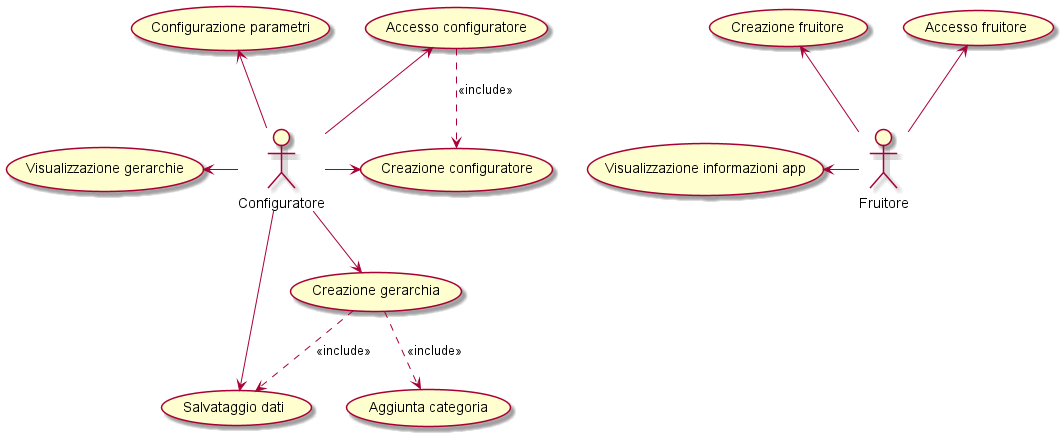
\includegraphics[width=0.9\textwidth]{imagesV2/Use case diagram-Version2.0.png}
\caption{\label{fig:Use Case 2}Diagramma UML dei casi d'uso - Versione 2}
\end{figure}\bigskip
\subsection{Diagramma UML delle classi}
In questa sezione sono stati riportati due diagrammi delle classi: il primo, in Figura \ref{fig:Class Diagram - v2}, rappresenta il diagramma delle classi dotato di tutte le dipendenze tra le classi, mentre il secondo, in Figura \ref{fig:Simplified Class Diagram - v2}, rappresenta il diagramma delle classi privato di alcune dipendenze esclusivamente al fine di renderne la comprensione più agevole.

Si tenga inoltre conto del fatto che le classi:
\begin{itemize}
    \item \texttt{CampoNativo}
    \item \texttt{Categoria}
    \item \texttt{Configuratore}
    \item \texttt{Fruitore}
    \item \texttt{Gerarchia}
    \item \texttt{Giorno}
    \item \texttt{InfoScambio}
    \item \texttt{IntervalloOrario}
    \item \texttt{Orario}
    \item \texttt{User}
    \item \texttt{UserDataStore}
\end{itemize}
implementano l'interfaccia \texttt{Serializable}, nonostante tale relazione non sia esplicitamente riportata nei diagrammi delle classi al fine di semplificare il layout dei diagrammi stessi.

\begin{figure}[h!]
    \centering
    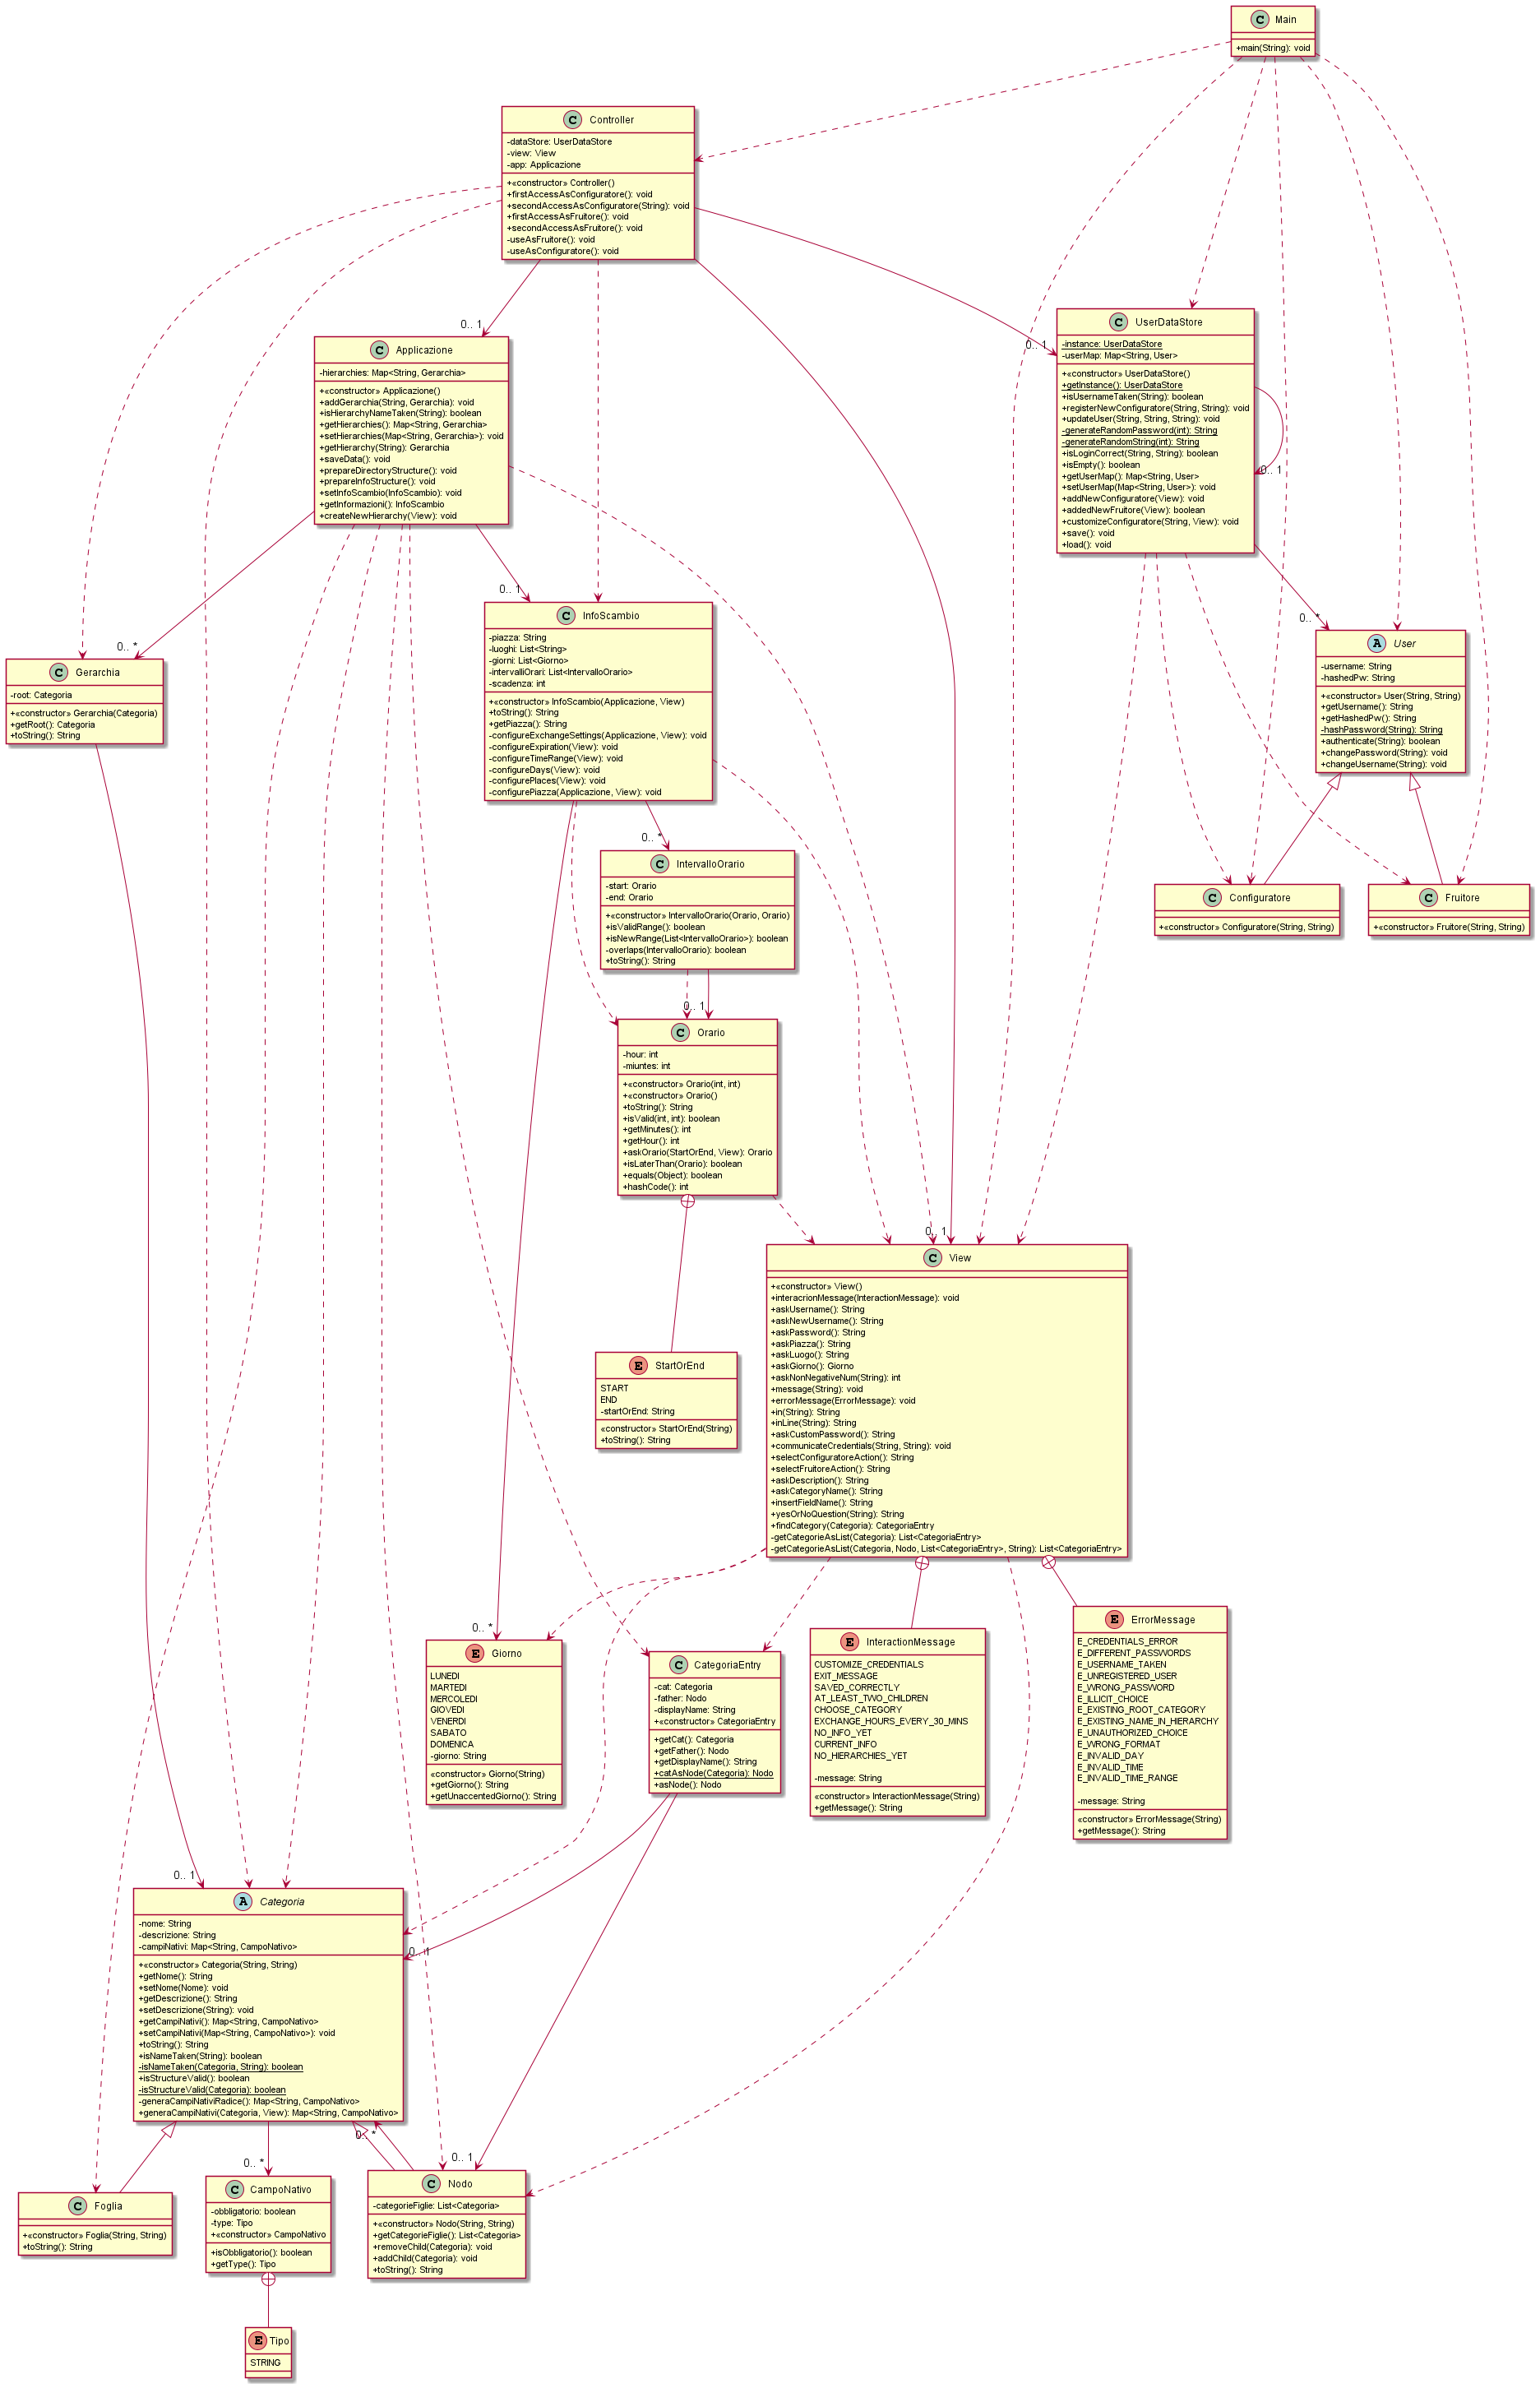
\includegraphics[width=\textwidth]{imagesV2/Class Diagram - Versione 2.0.png}
    \caption{\label{fig:Class Diagram - v2}Diagramma UML delle classi - Versione 2}
\end{figure} 

La classe \texttt{View} contiene i metodi (non indicati per esteso nel diagramma delle classi realizzato prima dell'effettiva stesura del codice) necessari per interagire e comunicare con l'utente, ricevendo i dati da lui inseriti oppure comunicando messaggi da parte del sistema.

La classe \texttt{UserDataStore} contiene i metodi necessari per la gestione dei dati relativi agli utenti che dovranno poi essere salvati in modo persistente. La classe ha il compito di gestire la registrazione di un nuovo utente, l'aggiornamento delle credenziali (se si tratta di un profilo Configuratore) e la verifica della correttezza delle informazioni introdotte in fase di login, oltre al salvataggio e al caricamento dei dati. 

La classe \texttt{User} è una classe astratta estesa dalla classe \texttt{Configuratore} e dalla classe \texttt{Fruitore}: ogni utente sarà dotato di username e password. La password, in particolare, viene salvata direttamente dopo aver effettuato l'hashing, in modo da garantire un livello di sicurezza basilare relativamente alle informazioni private degli utenti. La classe \texttt{User} è dotata di metodi per l'autenticazione dell'utente e per la modifica delle credenziali.

La classe \texttt{Applicazione} permette di tenere traccia delle gerarchie contenute nell'applicazione. 
Essa contiene infatti un metodo che verifica se il nome di una categoria radice di una gerarchia è già utilizzato dalla categoria radice di un'altra gerarchia, un metodo che permette di creare e aggiungere una nuova gerarchia, metodi che permettono di ottenere le gerarchie presenti nell'applicazione o di assegnare loro i valori desiderati, metodi che permettono di salvare i dati contenuti nelle gerarchie e di caricare i dati salvati durante gli utilizzi precedenti dell'applicazione.

La classe \texttt{Gerarchia} permette di tenere traccia del contenuto di ogni gerarchia: ogni gerarchia è caratterizzata da una categoria radice che, a seconda che sia istanza della classe \texttt{Foglia} o \texttt{Nodo}, può avere o meno delle sottocategorie (a loro volta istanze della classe \texttt{Foglia} o \texttt{Nodo}). 

La classe \texttt{Categoria} è una classe astratta che è estesa dalla classe \texttt{Foglia} e dalla classe \texttt{Nodo}. Ogni categoria è dotata di nome obbligatorio, descrizione facoltativa e un insieme di campi nativi (due dei quali presenti di default per la categoria radice di una gerarchia) ereditati poi da ogni categoria figlia di un nodo.
La classe \texttt{Nodo}, in particolare, è dotata di una lista di categorie figlie che possono a loro volta essere foglie o nodi. Per questo motivo la classe \texttt{Nodo} è dotata di metodi che permettono di aggiungere o rimuovere una categoria figlia e di un metodo che permette di ottenere tutte le categorie figlie.

La classe \texttt{CampoNativo} tiene traccia dell'obbligatorietà della compilazione di un campo, nativo o ereditato, relativo a una categoria e del tipo del campo (di default si tratta di stringhe). 

La classe \texttt{CategoriaEntry} tiene traccia dell'associazione tra una categoria e la sua categoria padre; essa contiene pertanto i metodi necessari a recuperare le informazioni relative a tale relazione (percorso dalla categoria radice alla categoria corrente, categoria padre e categoria corrente) e dei metodi per trasformare una categoria da Foglia a Nodo e associarla alla propria categoria padre.

La classe \texttt{Controller} contiene metodi per consentire l'accesso a un profilo Configuratore, differenziando tra il caso di registrazione e quello di accesso standard. Ognuno di questi metodi richiama poi uno o più ulteriori metodi che permettono l'utilizzo delle funzionalità a cui l'utente è autorizzato ad accedere; contiene inoltre metodi per consentire l'accesso a un profilo Fruitore, differenziando, come nel caso del configuratore, tra il caso di registrazione e quello di accesso, richiamando uno o più metodi che consentono di utilizzare tutte le funzionalità a cui l'utente è autorizzato ad accedere.

La classe \texttt{Main} contiene il solo metodo main che permette di interagire con l'applicazione selezionando l'azione da compiere tra accesso, registrazione o uscita dall'applicazione.

L'\textit{enum} \texttt{Giorno} gestisce l'elenco dei giorni della settimana.

La classe \texttt{InfoScambio} gestisce le informazioni di scambio che devono essere impostate dall'utente Configuratore.

La classe \texttt{IntervalloOrario} contiene metodi per validare la correttezza di un intervallo orario introdotto dall'utente, assicurandosi che l'intervallo non sia ancora stato inserito tra le informazioni di scambio e che non si sovrapponga ad altri intervalli già presenti.

La classe \texttt{Orario} contiene metodi per validare la correttezza di un singolo orario introdotto dall'utente, assicurando che esso sia nel formato \textit{[hh:mm]} e che i minuti possano essere o 00 oppure 30, in quanto gli scambi possono avvenire solo allo scoccare dell'ora o della mezz'ora.

\begin{figure}[h!]
    \centering
    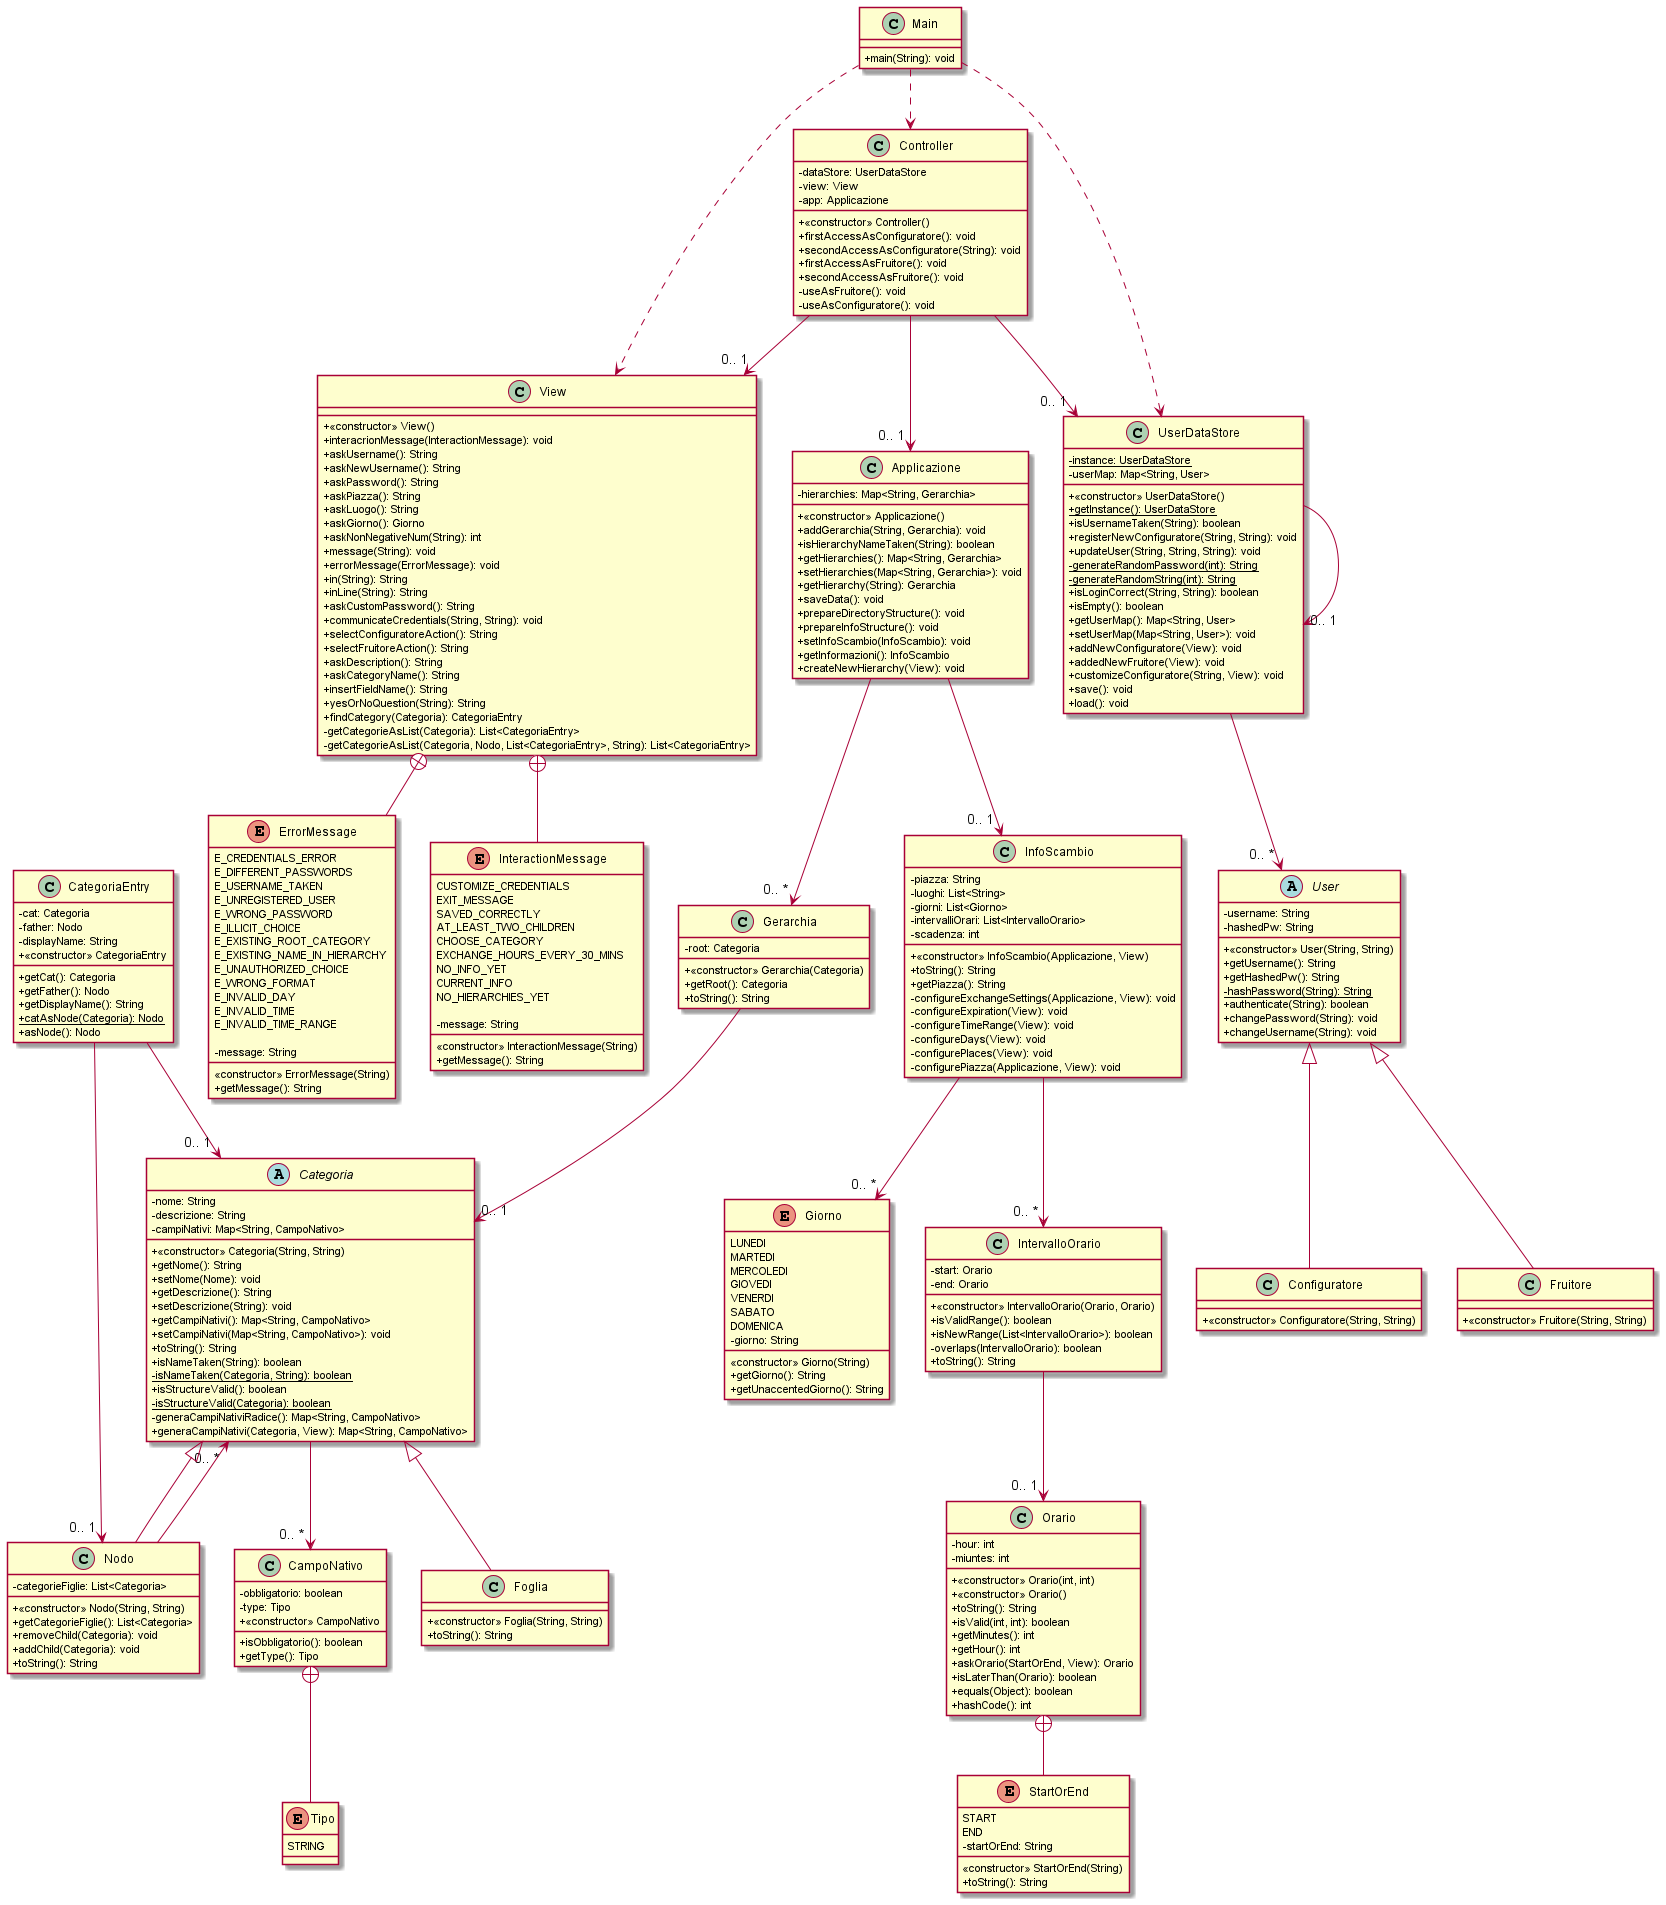
\includegraphics[width=\textwidth]{imagesV2/Vers2Parziale.png}
    \caption{\label{fig:Simplified Class Diagram - v2}Diagramma UML delle classi semplificato - Versione 2}
\end{figure}
\bigskip
\newpage
\subsection{Diagrammi UML comportamentali}
In questa sezione sono riportati alcuni diagrammi comportamentali a corredo dei diagrammi dei casi d'uso e UML delle classi che illustrano il funzionamento della seconda versione dell'applicazione.

I diagrammi UML riportati di seguito sono altamente descrittivi, in modo da essere utilizzabili per mostrare all'utente in maniera intuitiva il funzionamento dell'applicazione, pur rispettando le direttive UML.\bigskip

\newpage
\textbf{Diagramma degli Stati: Ciclo di vita dell'utente Configuratore}\newline
In Figura \ref{fig:State diagram 2.1} è rappresentato il ciclo di vita dell'utente Configuratore: a seconda dell'azione che esso intraprende nei confronti dell'applicazione il Configuratore si trova in un determinato stato.\newline L'accesso all'applicazione può avvenire o in qualità di primo accesso oppure come accesso ordinario: nel caso si tratti di un primo accesso il configuratore si riconduce allo stato \texttt{CreazioneProfilo} in cui avviene la creazione di un nuovo profilo Configuratore a cui segue un necessario cambio delle credenziali, mentre nel caso si tratti di un login ordinario l'utente accede direttamente al menu principale. \newline 
In tutti i passaggi di stato si considera la situazione ideale in cui non vi siano errori nell'esecuzione delle operazioni. Nel caso in cui si verifichino errori di esecuzione allora è lasciato sottinteso il passaggio attraverso uno stato di Errore prima di tornare al menu principale.

\begin{figure}[h!]
\centering
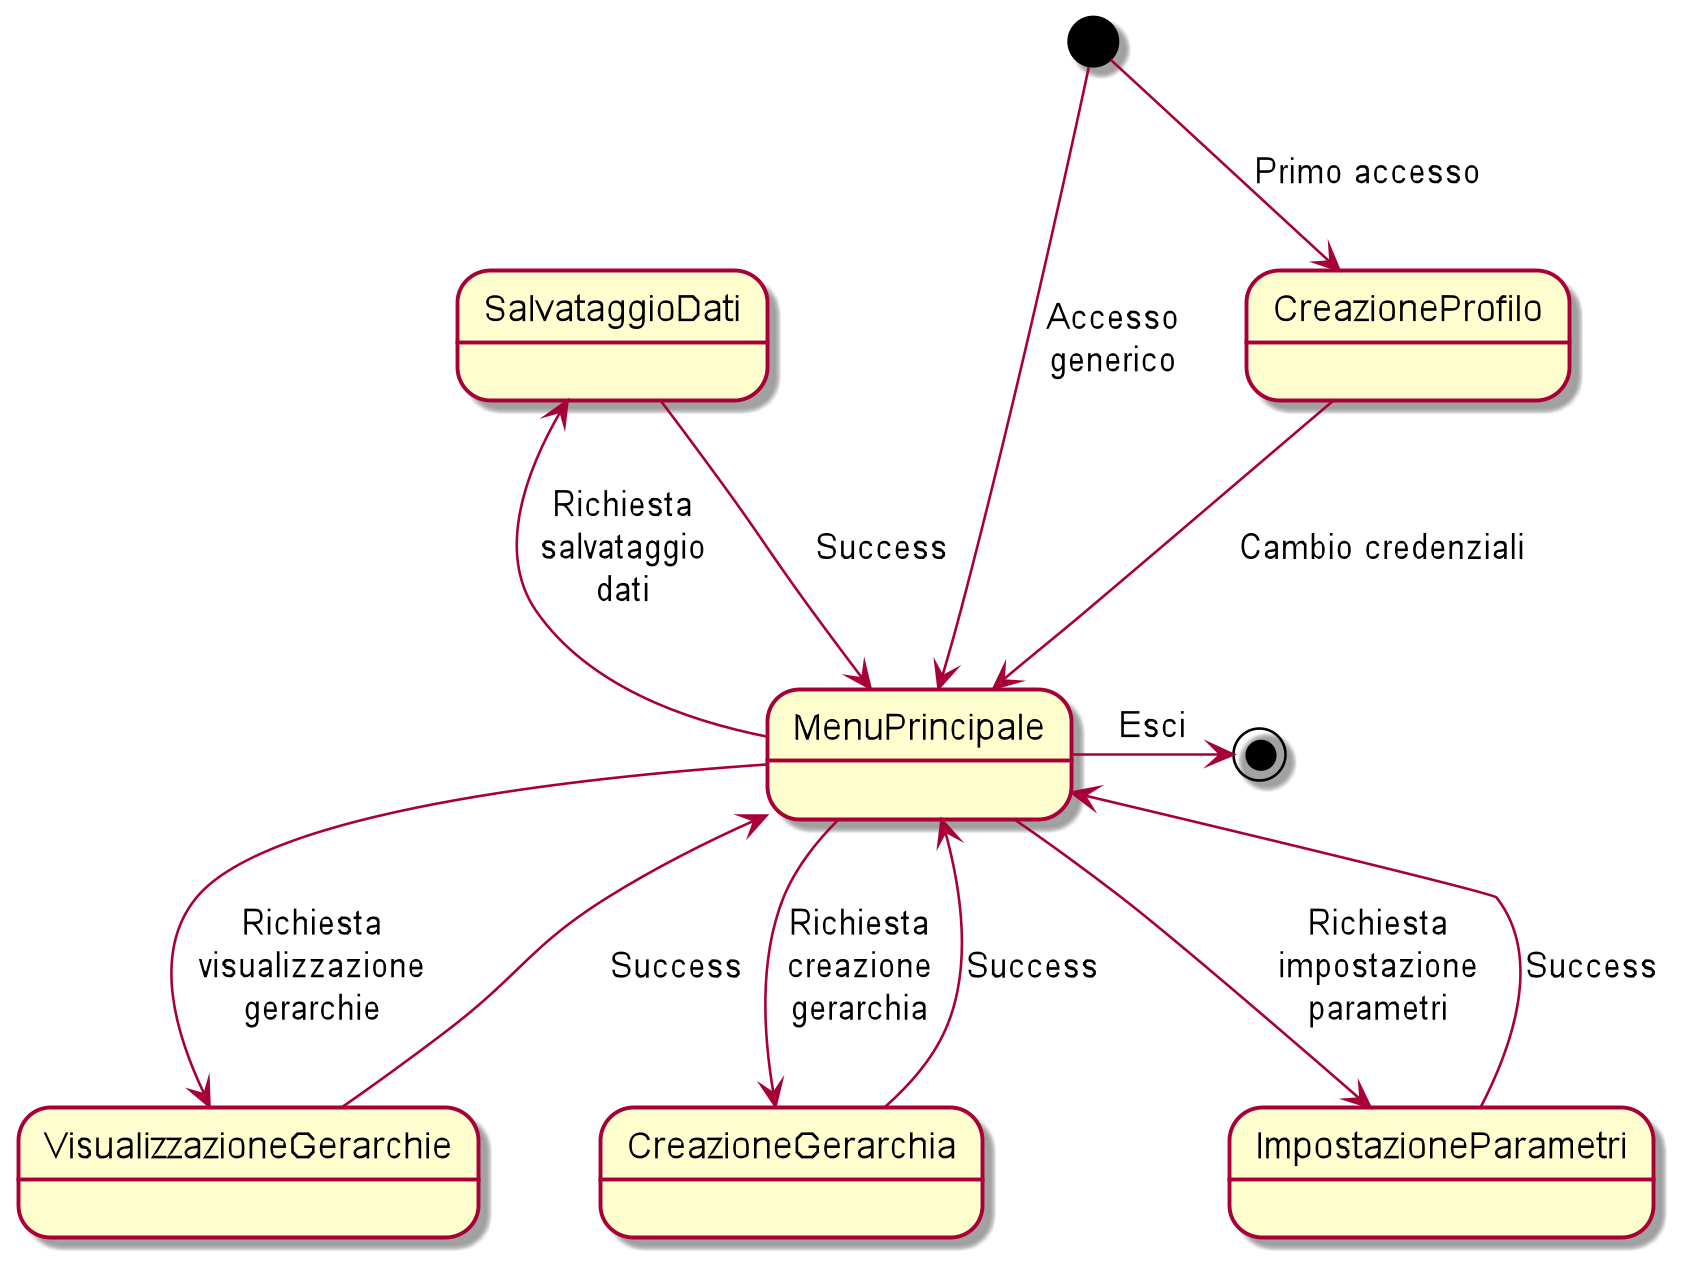
\includegraphics[width=0.7\textwidth]{imagesV2/State diagram-interazione configuratore v2.png}
\caption{\label{fig:State diagram 2.1}Ciclo di vita del Configuratore - Versione 2}
\end{figure}\bigskip

\textbf{Diagramma degli Stati: Ciclo di vita dell'utente Fruitore}\newline
In Figura \ref{fig:State diagram 2.2} è rappresentato il ciclo di vita dell'utente Fruitore: a seconda dell'azione che esso intraprende nei confronti dell'applicazione il Fruitore si trova in un determinato stato.\newline L'accesso all'applicazione può avvenire o in qualità di primo accesso oppure come accesso ordinario: nel caso si tratti di un primo accesso il Fruitore si riconduce allo stato \texttt{CreazioneProfilo} in cui avviene la creazione di un nuovo profilo Fruitore, mentre nel caso si tratti di un login ordinario l'utente accede direttamente al menu principale. \newline 
In tutti i passaggi di stato si considera la situazione ideale in cui non vi siano errori nell'esecuzione delle operazioni. Nel caso in cui si verifichino errori di esecuzione allora è lasciato sottinteso il passaggio attraverso uno stato di Errore prima di tornare al menu principale.

\begin{figure}[t!]
\centering
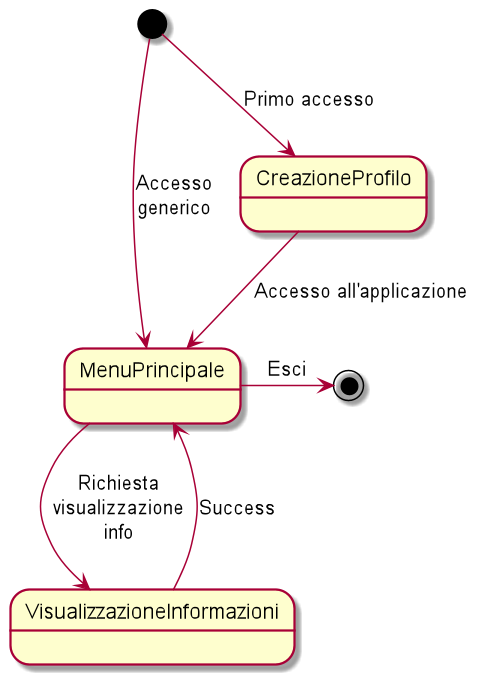
\includegraphics[width=0.5\textwidth, height=0.69\textwidth]{imagesV2/State diagram-interazione fruitore v2.png}
\caption{\label{fig:State diagram 2.2}Ciclo di vita del Fruitore - Versione 2}
\end{figure}\bigskip

\end{document}